
\documentclass[12pt, a4paper]{report}

\usepackage{epsfig}
\usepackage{subfigure}
%\usepackage{amscd}
\usepackage{amssymb}
\usepackage{graphicx}
%\usepackage{amscd}
\usepackage{amssymb}
\usepackage{subfiles}
\usepackage{framed}
\usepackage{subfiles}
\usepackage{amsthm, amsmath}
\usepackage{amsbsy}
\usepackage{framed}
\usepackage[usenames]{color}
\usepackage{listings}
\lstset{% general command to set parameter(s)
	basicstyle=\small, % print whole listing small
	keywordstyle=\color{red}\itshape,
	% underlined bold black keywords
	commentstyle=\color{blue}, % white comments
	stringstyle=\ttfamily, % typewriter type for strings
	showstringspaces=false,
	numbers=left, numberstyle=\tiny, stepnumber=1, numbersep=5pt, %
	frame=shadowbox,
	rulesepcolor=\color{black},
	,columns=fullflexible
} %
%\usepackage[dvips]{graphicx}
\usepackage{natbib}
\bibliographystyle{chicago}
\usepackage{vmargin}
% left top textwidth textheight headheight
% headsep footheight footskip
\setmargins{1.0cm}{0.75cm}{18.5 cm}{22cm}{0.5cm}{0cm}{1cm}{1cm}
%\voffset=-2.5cm
%\oddsidemargin=1cm
%\textwidth = 520pt

\renewcommand{\baselinestretch}{1.5}
\pagenumbering{arabic}
\theoremstyle{plain}
\newtheorem{theorem}{Theorem}[section]
\newtheorem{corollary}[theorem]{Corollary}
\newtheorem{ill}[theorem]{Example}
\newtheorem{lemma}[theorem]{Lemma}
\newtheorem{proposition}[theorem]{Proposition}
\newtheorem{conjecture}[theorem]{Conjecture}
\newtheorem{axiom}{Axiom}
\theoremstyle{definition}
\newtheorem{definition}{Definition}[section]
\newtheorem{notation}{Notation}
\theoremstyle{remark}
\newtheorem{remark}{Remark}[section]
\newtheorem{example}{Example}[section]
\renewcommand{\thenotation}{}
\renewcommand{\thetable}{\thesection.\arabic{table}}
\renewcommand{\thefigure}{\thesection.\arabic{figure}}
\title{Research notes: linear mixed effects models}
\author{ } \date{ }


\begin{document}
	\author{Kevin O'Brien}
	\title{Mixed Models for Method Comparison Studies}
	\tableofcontents
	
	\chapter{Fitting MCS Models with R}
	%========================================================= %
\section{Computation of LMEs using R} \cite{PB} advises how to
implement LME models in statistical software (ostensibly for S and
S PLUS, but R is very similar). When tackling linear mixed effects
models using the R language, a statistician can call upon the
\emph{lme} command found in the \emph{nlme} package.This command
fits a LME model to the data set using either Maximum Likelihood
(ML) or Restricted Maximum Likelihood (REML). ML may be referred
to as 'full maximum likelihood' estimation.

The first two arguments for \emph{lme} are \emph{fixed} and
\emph{data}, which give the model for the expected responses (i.e.
the fixed part of the model), and the data that themodel should be
fitted from. The next argument is  \emph{random}, a one-sided
formula which describes the random effects, and the grouping
structure for the model. The  \emph{method} argument can specify
whether to use 'REML', the default setting, or 'ML'.

\citet{PB} describes an experiment whereby the productivity of six
randomly chosen workers are assessed three times on each of three
machines, yielding the 54 observations in the following table.


% latex table generated in R 2.9.2 by xtable 1.5-5 package
% Wed Sep 16 13:56:04 2009
\begin{table}[h!]
	\begin{center}
		\begin{tabular}{|c|c|c|c||c|c|c|c|}
			\hline
			Observation & Worker & Machine & score & Observation & Worker & Machine & score \\
			\hline
			1 & 1 & A & 52.00 &	28 & 4 & B & 63.20 \\
			2 & 1 & A & 52.80 &	  29 & 4 & B & 62.80 \\
			3 & 1 & A & 53.10 &	  30 & 4 & B & 62.20 \\
			4 & 2 & A & 51.80 &	  31 & 5 & B & 64.80 \\
			5 & 2 & A & 52.80 &	  32 & 5 & B & 65.00 \\
			6 & 2 & A & 53.10 &	  33 & 5 & B & 65.40 \\
			7 & 3 & A & 60.00 &	  34 & 6 & B & 43.70 \\
			8 & 3 & A & 60.20 &	  35 & 6 & B & 44.20 \\
			9 & 3 & A & 58.40 &	  36 & 6 & B & 43.00 \\
			10 & 4 & A & 51.10 &	  37 & 1 & C & 67.50 \\
			11 & 4 & A & 52.30 &	  38 & 1 & C & 67.20 \\
			12 & 4 & A & 50.30 &	  39 & 1 & C & 66.90 \\
			13 & 5 & A & 50.90 &	  40 & 2 & C & 61.50 \\
			14 & 5 & A & 51.80 &	  41 & 2 & C & 61.70 \\
			15 & 5 & A & 51.40 &	  42 & 2 & C & 62.30 \\
			16 & 6 & A & 46.40 &	  43 & 3 & C & 70.80 \\
			17 & 6 & A & 44.80 &	  44 & 3 & C & 70.60 \\
			18 & 6 & A & 49.20 &	  45 & 3 & C & 71.00 \\
			19 & 1 & B & 62.10 &	  46 & 4 & C & 64.10 \\
			20 & 1 & B & 62.60 &	  47 & 4 & C & 66.20 \\
			21 & 1 & B & 64.00 &	  48 & 4 & C & 64.00 \\
			22 & 2 & B & 59.70 &	  49 & 5 & C & 72.10 \\
			23 & 2 & B & 60.00 &	  50 & 5 & C & 72.00 \\
			24 & 2 & B & 59.00 &	  51 & 5 & C & 71.10 \\
			25 & 3 & B & 68.60 &	  52 & 6 & C & 62.00 \\
			26 & 3 & B & 65.80 &	  53 & 6 & C & 61.40 \\
			27 & 3 & B & 69.70 &	  54 & 6 & C & 60.50 \\
			
			\hline
		\end{tabular}
		\caption{Machines Data , Pinheiro Bates}
	\end{center}
\end{table}
(Overall mean score = $59.65$, mean on machine A = $52.35$ , mean
on machine B = $60.32$, mean on machine C = $66.27$)


The `worker' factor is modelled with random effects($u_{i}$),
whereas the `machine' factor is modelled with fixed effects
($\beta_{j}$). Due to the repeated nature of the data, interaction
effects between these factors are assumed to be extant, and shall
be examined accordingly. The interaction effect in this case
($\tau_{ij}$) describes whether the effect of changing from one
machine to another is different for each worker. The productivity
score $y_{ijk}$ is the $k$th observation taken on worker $i$ on
machine $j$, and is formulated
as follows;

\begin{equation}
y_{ijk} = \beta_{j} + u_{i} + \tau_{ij} + \epsilon_{ijk}
\end{equation}
%\begin{equation*}
%	u_{i} \sim N(0, \sigma^{2}_{u}), \epsilon_{ijk} \sim N(0,
%	\sigma^{2}), \tau_{i} \sim N(0, \sigma^{2}_{\tau})
%\end{equation*}

The `nlme' package is incorporated into the R programming to
perform linear mixed model calculations. For the `Machines' data,
\citet{pb} use the following code, with the hierarchical structure
specified in the last argument.
\begin{verbatim}
lme(score~Machine, data=Machines, random=~1|Worker/Machine)
\end{verbatim}


The output of the R computation is given below.
\begin{verbatim}
Linear mixed-effects model fit by REML
Data: Machines
Log-restricted-likelihood: -107.8438
Fixed: score ~ Machine
(Intercept)    MachineB    MachineC
52.355556    7.966667   13.916667

Random effects:
Formula: ~1 | Worker
(Intercept)
StdDev:     4.78105

Formula: ~1 | Machine %in% Worker
(Intercept)  Residual
StdDev:    3.729532 0.9615771

Number of Observations: 54 Number of Groups:
Worker Machine %in% Worker
6                  18

\end{verbatim}


The crucial pieces of information given in the programme output
are the estimates of the intercepts for each of the three
machines. Machine A, which is treated as a control case, is
estimated to have an intercept of 52.35. The intercept estimates
for machines B and C are found to be $60.32$ and $66.27$ (by
adding the values 7.96 and 13.91 to 52.35 respectively). Estimate
for the variance components are also given; $\sigma^{2}_{u} =
(4.78)^{2}$ , $\sigma^{2}_{\tau} = (3.73)^{2}$ and
$\sigma^{2}_{\epsilon} = (0.96)^{2}$.

%%%%%%%%%%%%%%%%%%%%%%%%%%%%%%%%%%%%%%%%%%%%%%%%%%%%%%%%%%%%%%%%%%%%%%%%%%%%%%%%%%%%%%%%%%%%%%%%%%% MODEL SELECTION



	\section{Introduction}
	
	\citet{AARoy20092009} uses an approach based on linear mixed effects (LME) models for the purpose of comparing the agreement between two methods of measurement, where replicate measurements on items, typically individuals, by both methods are available. She provides three tests of hypothesis appropriate for evaluating the agreement between the two methods of measurement under this sampling scheme. These tests consider null hypotheses that assume: absence of inter-method bias; equality of between-subject variabilities of the two methods; equality of within-subject variabilities of the two methods. By inter-method bias we mean that a systematic difference exists between observations recorded by the two methods. Differences in between-subject variabilities of the two methods arise when one method is yielding average response levels for individuals than are more variable than the average response levels for the same sample of individuals taken by the other method.  Differences in within-subject variabilities of the two methods arise when one method is yielding responses for an individual than are more variable than the responses for this same individual taken by the other method. The two methods of measurement can be considered to agree, and subsequently can be used interchangeably, if all three null hypotheses are true.
	
	\subsection{Model Specification}
	Let $y_{mir} $ be the $r$th replicate measurement on the $i$th item by the $m$th method, where $m=1,2,$ $i=1,\ldots,N,$ and $r = 1,\ldots,n_i.$ When the design is balanced and there is no ambiguity we can set $n_i=n.$ The LME model can be written
	\begin{equation}
	y_{mir} = \beta_{0} + \beta_{m} + b_{mi} + \epsilon_{mir}.
	\end{equation}
	Here $\beta_0$ and $\beta_m$ are fixed-effect terms representing, respectively, a model intercept and an overall effect for method $m.$ The $b_{1i}$ and $b_{2i}$ terms represent random effect parameters corresponding to the two methods, having $\mathrm{E}(b_{mi})=0$ with $\mathrm{Var}(b_{mi})=g^2_m$ and $\mathrm{Cov}(b_{mi}, b_{m^\prime i})=g_{12}.$ The random error term for each response is denoted $\epsilon_{mir}$ having $\mathrm{E}(\epsilon_{mir})=0$, $\mathrm{Var}(\epsilon_{mir})=\sigma^2_m$, $\mathrm{Cov}(b_{mir}, b_{m^\prime ir})=\sigma_{12}$, $\mathrm{Cov}(\epsilon_{mir}, \epsilon_{mir^\prime})= 0$ and $\mathrm{Cov}(\epsilon_{mir}, \epsilon_{m^\prime ir^\prime})= 0.$
	When two methods of measurement are in agreement, there is no significant differences between $\beta_1$ and $\beta_2,$ $g^2_1 $ and$ g^2_2$, and $\sigma^2_1 $ and$ \sigma^2_2$.
	\bigskip
	
	% Complete paragraph by specifying variances and covariances for epsilons.
	% I thing that these are your sigmas?
	% Also, state equality of the parameters in this model when each of the three hypotheses above are true.
	
	
	\newpage
	
	\section{Model terms}
	It is important to note the following characteristics of this model.
	\begin{itemize}
		\item Let the number of replicate measurements on each item $i$ for both methods be $n_i$, hence $2 \times n_i$ responses. However, it is assumed that there may be a different number of replicates made for different items. Let the maximum number of replicates be $p$. An item will have up to $2p$ measurements, i.e. $\max(n_{i}) = 2p$.
		
		% \item $\boldsymbol{y}_i$ is the $2n_i \times 1$ response vector for measurements on the $i-$th item.
		% \item $\boldsymbol{X}_i$ is the $2n_i \times  3$ model matrix for the fixed effects for observations on item $i$.
		% \item $\boldsymbol{\beta}$ is the $3 \times  1$ vector of fixed-effect coefficients, one for the true value for item $i$, and one effect each for both methods.
		
		\item Later on $\boldsymbol{X}_i$ will be reduced to a $2 \times 1$ matrix, to allow estimation of terms. This is due to a shortage of rank. The fixed effects vector can be modified accordingly.
		\item $\boldsymbol{Z}_i$ is the $2n_i \times  2$ model matrix for the random effects for measurement methods on item $i$.
		\item $\boldsymbol{b}_i$ is the $2 \times  1$ vector of random-effect coefficients on item $i$, one for each method.
		\item $\boldsymbol{\epsilon}$  is the $2n_i \times  1$ vector of residuals for measurements on item $i$.
		\item $\boldsymbol{G}$ is the $2 \times  2$ covariance matrix for the random effects.
		\item $\boldsymbol{R}_i$ is the $2n_i \times  2n_i$ covariance matrix for the residuals on item $i$.
		\item The expected value is given as $\mbox{E}(\boldsymbol{y}_i) = \boldsymbol{X}_i\boldsymbol{\beta}.$ \citep{hamlett}
		\item The variance of the response vector is given by $\mbox{Var}(\boldsymbol{y}_i)  = \boldsymbol{Z}_i \boldsymbol{G} \boldsymbol{Z}_i^{\prime} + \boldsymbol{R}_i$ \citep{hamlett}.
	\end{itemize}
	
	
	\section{Fitting Models with the LME4 R package}
	Two LME models are fitted to the data, one using the nlme package, one with the lme4 package. These models shall be called ``blood.nlme" and ``blood.lme4" respectively.
	In both cases the method is characterized by a fixed effect, while there is a random effect for each subject.
	This random effect accounts for the replicate measurements associated with each subject.
	The differences between the estimate provided by the respective models are negligible, due to the simplicity of the model specification.
	
	
	Maximum likelihood or restricted maximum likelihood (REML) estimates of the parameters in linear mixed-effects models can be determined using the \texttt{lmer} function in the lme4 package for R. As for most model-fitting functions in R, the model is described in an \texttt{lmer} call by a formula, in this case including both fixed- and random-effects terms. 
	
	The formula and data together determine a numerical representation of the model from which the profiled deviance or the profiled REML criterion can be evaluated as a function of some of the model parameters. The appropriate criterion is optimized, using one of the constrained optimization functions in \texttt{R}, to provide the parameter estimates. We describe the structure of the model, the steps in evaluating the profiled deviance or REML criterion, and the structure of classes or types that represents such a model. 
	
	Sufficient detail is included to allow specialization of these structures by users who wish to write functions to fit specialized linear mixed models, such as models incorporating pedigrees or smoothing splines, that are not easily expressible in the formula language used by lmer.
	
	
	\begin{description}
		\item[\texttt{y}] : Response variable
		\item[\texttt{method}] : Method of Measurement
		\item[\texttt{subject}] : Subject
		\item[\texttt{MCSdata}] 
	\end{description}
	\begin{framed}
		\begin{verbatim}
		library(lme4)
		
		MCS.lme4 <- lmer(y ~ method-1 + (1|subject) , data=MCSdata)
		\end{verbatim}
	\end{framed}
	\newpage
	
	%=====================%
	\subsection{Important Consideration for MCS}
	
	The key issue is that \texttt{nlme} allows for the particular specification of ARoy2009's Model, specifically direct specification of the VC matrices for within subject and between subject residuals.
	
	The \texttt{lme4} package does not allow for ARoy2009's Model, for reasons that will identified shortly.
	To advance the ideas that eminate from ARoy2009s' paper, one is required to use the \texttt{nlme} context. However, to take advantage of the infrastructure already provided for \texttt{lme4} models, one may change the research question away from that of ARoy2009's paper. 
	To this end, an exploration of what textbf{influence.ME} can accomplished is merited.
	%===================================================================================================%
	%-----------------------------------------------------------------------------------------%
	\subsection{Studentized Residuals}
	Standardization is not possible in practice. Studentized residuals are residuals divided by the estimated standard estimation.
	[Gregoire,Schabenberger, Barrett (1995)]
	
	\[\boldsymbol{r}_{m} = \boldsymbol{Y} -  \boldsymbol{X} \boldsymbol{\hat{\beta}} \]
	
	\[\boldsymbol{r}_{c} = \boldsymbol{Y} -  \boldsymbol{X} \boldsymbol{\hat{\beta}} -  \boldsymbol{Z} \boldsymbol{\hat{\gamma}}\]
	
	For the individual observation the raw studentized and pearson type residuals are computed as follows:
	\[r_{mi} =Y_{i} -X^{\prime} \boldsymbol{\hat{\beta}}\]
	
	\[r_{ci} = r_{mi} - Y_{i} - z_{i}^{\prime} \boldsymbol{\hat{\gamma}}\]
	
	
	\subsection{Residuals in the Blood Data Example}
	The fitted model used in the Blood data example, \texttt{JS.ARoy20091}, was fitted using the \texttt{lme()} function from the nlme package, and as such, is stored as an \texttt{lme} object. The \texttt{residual} functions extracts residuals of a fitted LME model, depending on the type of residual required.
	
	For an lme object, the residuals at level $i$ are obtained by subtracting the fitted levels at that level from the response vector (and dividing by the estimated within-group standard error, if \texttt{type="pearson"}). The Pearson residual is the raw residual divided by the square root of the variance function (here, the Within-group standard error for both methods, 6.11 and 9.11 respectively). The fitted values at level $i$ are obtained by adding together the population fitted values (based only on the fixed effects estimates) and the estimated contributions of the random effects to the fitted values at grouping levels less or equal to $i$.
	
	\begin{description}
		\item["\texttt{response}"]: the “raw” residuals (\textit{observed - fitted}) are used. This is the default option.
		\item["\texttt{pearson}"]: the standardized residuals (raw residuals divided by the corresponding standard errors) are used; 
		\item["\texttt{normalized}"]: the normalized residuals (standardized residuals pre-multiplied by the inverse square-root factor of the estimated error correlation matrix) are used.
	\end{description}
	
	\begin{framed}
		\begin{verbatim}
		data.frame( response = resid(JS.ARoy20091, type = "response"), 
		pearson  = resid(JS.ARoy20091, type = "pearson"), 
		normalized = resid(JS.ARoy20091, type = "normalized") )
		\end{verbatim}
	\end{framed}
	
	\begin{verbatim}
	response      pearson    normalized
	1    -4.65805902 -0.761587227 -0.7615872269
	2    -0.88701342 -0.145025661  0.0776238081
	3    -5.16580898 -0.844603753 -0.8446037530
	4     2.29041830  0.374480726  0.6450898404
	5     7.87508366  1.287567009  1.2875670086
	6    -6.57048659 -1.074266908 -1.5090772378
	...........................................
	\end{verbatim}
	For the $J$ observations, the variance is 6.116252 whereas for the $S$ observations, the denominator is 9.118144. (with the expected ratio of  1.490806)
	
	
	\begin{framed}
		\begin{verbatim}
		> pearson %>%
		+   as.numeric %>% 
		+   matrix(nrow=85) %>%
		+   round(4) 
		[,1]    [,2]    [,3]    [,4]    [,5]    [,6]
		[1,] -0.7616  0.2194  0.3829 -0.2983  0.3597 -0.0790
		[2,] -0.1450  0.1820 -0.1450 -0.5014  0.1567  0.2663
		[3,] -0.8446  0.4634  0.1364 -0.1630 -0.2727  0.1660
		[4,]  0.3745 -0.2795 -0.2795 -0.2658 -0.2658  0.6115
		[5,]  1.2876 -0.6744 -0.6744  0.8935 -0.0935 -0.8612
		[6,] -1.0743  1.8687 -0.7473 -0.0383  0.2908 -0.3673
		...........................................
		
		\end{verbatim}
	\end{framed}
	
	We can plot the residuals against the fitted values, to assess the assumption of constant variance. 
	\begin{framed}
		\begin{verbatim}
		# standardized residuals versus fitted values 
		plot(JS.ARoy20091, resid(., type = "pearson") ~ fitted(.) , 
		abline = 0, id = 0.05)
		\end{verbatim}
	\end{framed}
	\begin{figure}[h!]
		\centering
		\includegraphics[width=0.9\linewidth]{images/Residuals-JS-roy}
		\caption{}
		\label{fig:Residuals-JS-ARoy2009}
	\end{figure}
	\subsection{Residual Plots}
	A residual plot is a graph that shows the residuals on the vertical axis and the independent variable on the horizontal axis. If the points in a residual plot are randomly dispersed around the horizontal axis, a linear regression model is appropriate for the data; otherwise, a non-linear model is more appropriate.
	
	\begin{framed}
		\begin{verbatim}
		par(mfrow=c(1,2))
		qqnorm((resid(JS.ARoy20091)[1:255]),
		pch="*",col="red",
		ylim=c(-40,40),
		main="Method J")
		qqline(resid(JS.ARoy20091)[1:255],col="blue")
		qqnorm((resid(JS.ARoy20091)[256:510]),
		pch="*",col="red",
		ylim=c(-40,40),
		main="Method S")
		qqline(resid(JS.ARoy20091)[256:510],col="blue")
		par(mfrow=c(1,1))
		\end{verbatim}	
	\end{framed}
	
	
	\begin{figure}[h!]
		\centering
		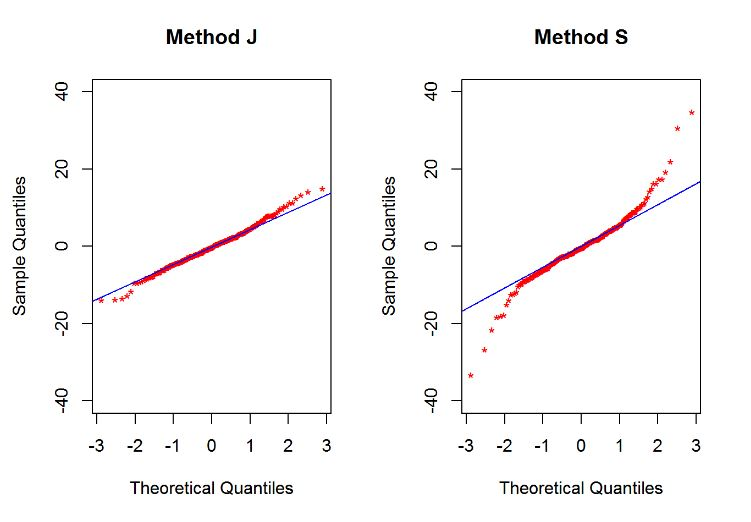
\includegraphics[width=1.1\linewidth]{images/Resid-newplot2}
		\caption{}
		\label{fig:Resid-newplot2}
	\end{figure}
	
	
	\begin{figure}[h!]
		\centering
		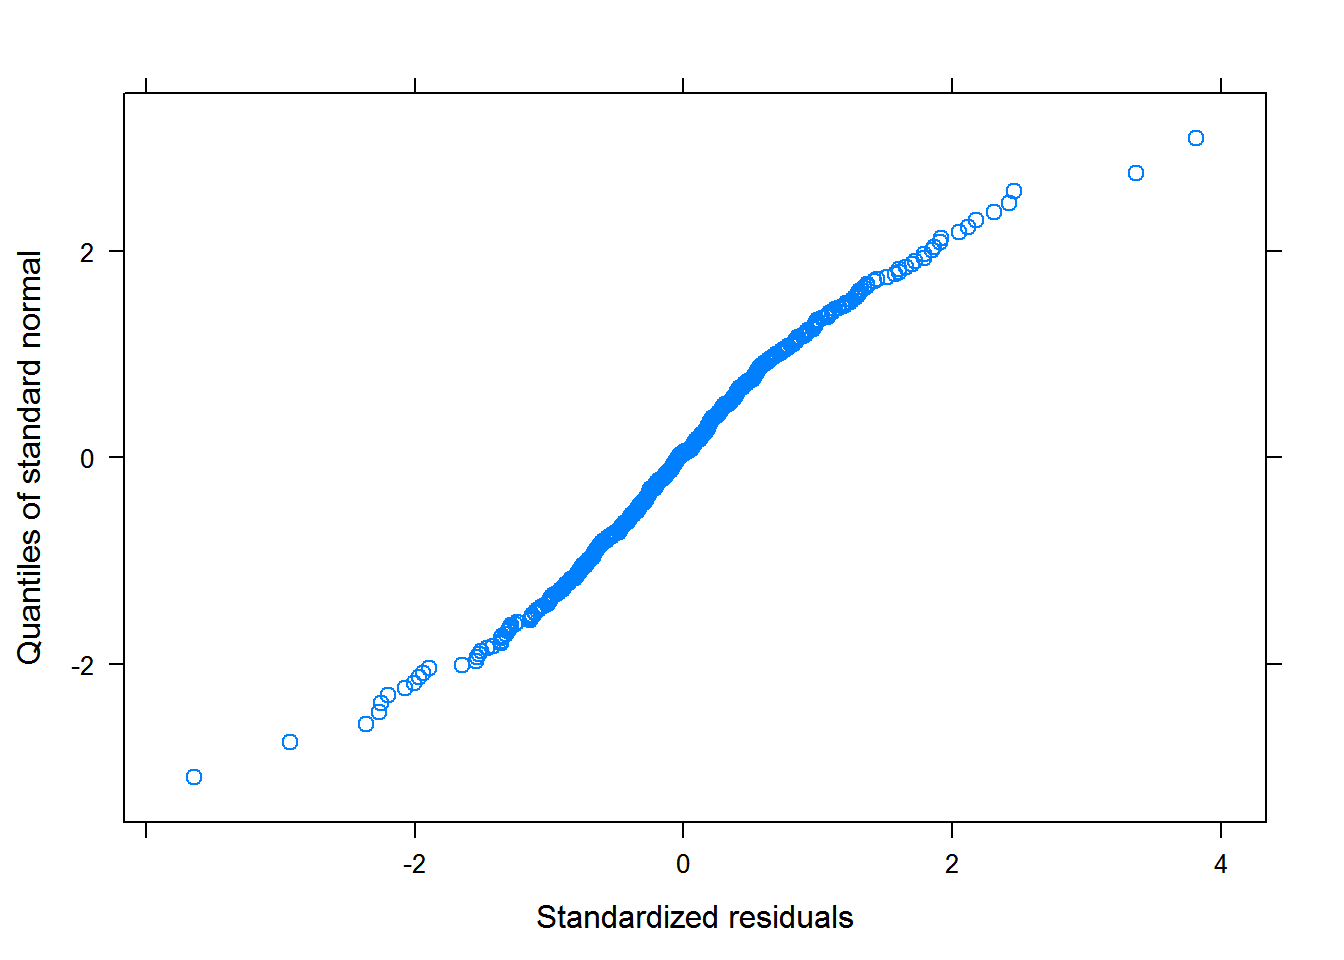
\includegraphics[width=0.9\linewidth]{images/ResidPlot3}
		\label{fig:ResidPlot3}
	\end{figure}
	
	This code will allow you to make QQ plots for each level of the random effects.  LME models assume that not only the within-cluster residuals are normally distributed, but that each level of the random effects are as well. Depending on the model, you can vary the level from 0, 1, 2 and so on
	\begin{framed}
		\begin{verbatim}
		qqnorm(JS.ARoy20091, ~ranef(.))
		
		# 	qqnorm(JS.ARoy20091, ~ranef(.,levels=1)
		\end{verbatim}
	\end{framed}
	\begin{figure}[h!]
		\centering
		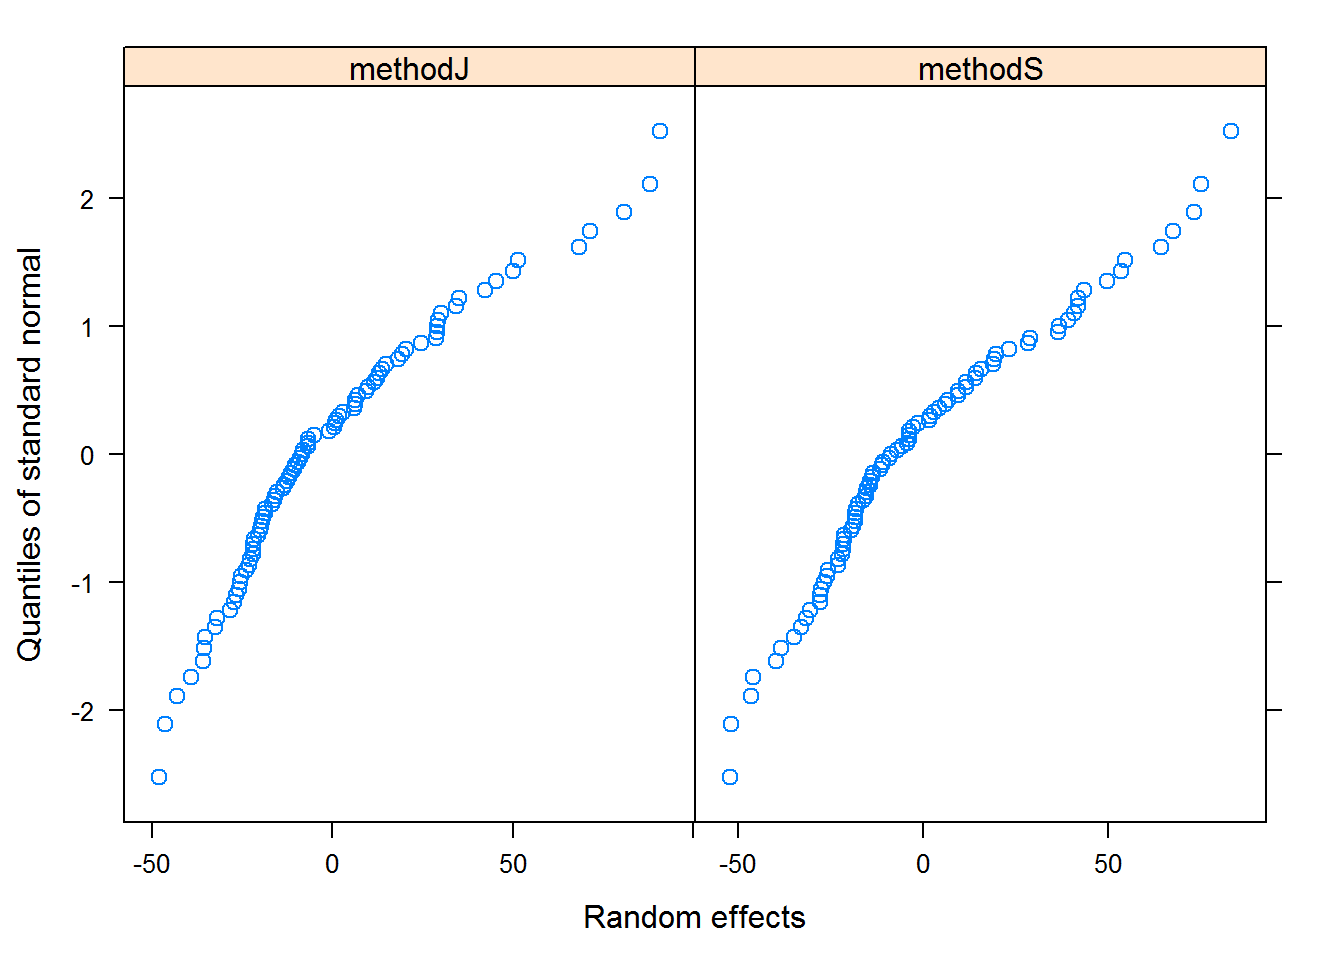
\includegraphics[width=0.9\linewidth]{images/ResidPlot2}
		\caption{}
		\label{fig:ResidPlot2}
	\end{figure}	
	
	
	\section{Model Terms for ARoy2009's Techniques}
	\begin{enumerate}
		\item $\boldsymbol{b}_{i}$ is a $m-$dimensional vector comprised of
		the random effects.
		\begin{equation}
		\boldsymbol{b}_{i} = \left( \begin{array}{c}
		b_{1i} \\
		b_{21}  \\
		\end{array}\right)
		\end{equation}
		
		\item $\boldsymbol{V}$ represents the correlation matrix of the replicated measurements on a given method.
		$\boldsymbol{\Sigma}$ is the within-subject VC matrix.
		
		\item $\boldsymbol{V}$ and $\boldsymbol{\Sigma}$ are positive
		definite matrices. The dimensions of $\boldsymbol{V}$ and
		$\boldsymbol{\Sigma}$ are $3 \times 3 ( = p \times p )$ and $ 2 \times
		2 (= k \times k)$.
		
		\item It is assumed that $\boldsymbol{V}$ is the same for both methods and $\boldsymbol{\Sigma}$ is
		the same for all replications.
		
		\item $\boldsymbol{V} \bigotimes \boldsymbol{\Sigma}$ creates a $ 6 \times 6 ( = kp \times
		kp)$ matrix.
		$\boldsymbol{R}_{i}$ is a sub-matrix of this.
	\end{enumerate}
	
	\section{Demonstration of ARoy2009's testing}
	ARoy2009 provides three case studies, using data sets well known in method comparison studies, to demonstrate how the methodology should be used. The first two examples used are from the `blood pressure' data set introduced by \citet{BA99}. The data set is a tabulation of simultaneous measurements of systolic blood pressure were made by each of two experienced observers (denoted `J' and `R') using a sphygmomanometer and by a semi-automatic blood pressure monitor (denoted `S'). Three sets of readings were made in quick succession. ARoy2009 compares the `J' and `S' methods in his first example, and the `R' and `S' methods in his second.
	
	The inter-method bias between the two method is found to be $15.62$ , with a $t-$value of $-7.64$, with a $p-$value of less than $0.0001$. Consequently there is a significant inter-method bias present between methods $J$ and $S$, and the first of the ARoy2009's three agreement criteria is unfulfilled.
	
	Next, the first variability test is carried out, yielding maximum likelihood estimates of the between-subject variance covariance matrix, for both the null model, in compound symmetry (CS) form, and the alternative model in symmetric (symm) form. These matrices are determined to be as follows;
	\[
	\boldsymbol{\hat{D}}_{CS} = \left( \begin{array}{cc}
	946.50 & 784.32  \\
	784.32 & 946.50  \\
	\end{array}\right),
	\hspace{1.5cm}
	\boldsymbol{\hat{D}}_{Symm} = \left( \begin{array}{cc}
	923.98 & 785.24  \\
	785.24 & 971.30  \\
	\end{array}\right).
	\]
	
	A likelihood ratio test is perform to compare both candidate models. The log-likelihood of the null model is $-2030.7$, and for the alternative model $-2030.8$. The test statistic, presented with greater precision than the log-likelihoods, is $0.1592$. The $p-$value is $0.6958$. Consequently we fail to reject the null model, and by extension, conclude that the hypothesis that methods $J$ and $S$ have the same between-subject variability. Thus the second of the criteria is fulfilled.
	
	The second variability test determines maximum likelihood estimates of the within-subject variance covariance matrix, for both the null model, in CS form, and the alternative model in symmetric form.
	
	\[
	\boldsymbol{\hat{\Lambda}_{CS}} = \left( \begin{array}{cc}
	60.27  & 16.06  \\
	16.06  & 60.27  \\
	\end{array}\right),
	\hspace{1.5cm}
	\boldsymbol{\hat{\Lambda}}_{Symm} = \left( \begin{array}{cc}
	37.40 & 16.06  \\
	16.06 & 83.14  \\
	\end{array}\right).
	\]
	
	Again, A likelihood ratio test is perform to compare both candidate models. The log-likelihood of the alternative model model is $-2045.0$. As before, the null model has a log-likelihood of $-2030.7$. The test statistic is computed as $28.617$, again presented with greater precision. The $p-$value is less than $0.0001$. In this case we reject the null hypothesis of equal within-subject variability. Consequently the third of ARoy2009's criteria is unfulfilled.
	The coefficient of repeatability for methods $J$ and $S$ are found to be 16.95 mmHg and 25.28 mmHg respectively.
	
	The last of the three variability tests is carried out to compare the overall variabilities of both methods.
	With the null model the MLE of the within-subject variance covariance matrix is given below. The overall variabilities for the null and alternative models, respectively, are determined to be as follows;
	\[
	\boldsymbol{\hat{\Sigma}}_{CS} = \left( \begin{array}{cc}
	1007.92  & 801.65  \\
	801.65  & 1007.92  \\
	\end{array}\right),
	\hspace{1.5cm}
	\boldsymbol{\hat{\Sigma}}_{Symm} = \left( \begin{array}{cc}
	961.38 & 801.40  \\
	801.40 & 1054.43  \\
	\end{array}\right),
	\]
	
	The log-likelihood of the alternative model model is $-2045.2$, and again, the null model has a log-likelihood of $-2030.7$. The test statistic is $28.884$, and the $p-$value is less than $0.0001$. The null hypothesis, that both methods have equal overall variability, is rejected. Further to the second variability test, it is known that this difference is specifically due to the difference of within-subject variabilities.
	
	Lastly, ARoy2009 considers the overall correlation coefficient. The diagonal blocks $\boldsymbol{\hat{r}_{\Omega}}_{ii}$ of the correlation matrix indicate an overall coefficient of $0.7959$. This is less than the threshold of 0.82 that ARoy2009 recommends.
	
	\[
	\boldsymbol{\hat{r}_{\Omega}}_{ii} = \left( \begin{array}{cc}
	1  & 0.7959  \\
	0.7959  & 1  \\
	\end{array}\right)
	\]
	
	The off-diagonal blocks of the overall correlation matrix $\boldsymbol{\hat{r}_{\Omega}}_{ii'}$ present the correlation coefficients further to \citet{hamlett}.
	\[
	\boldsymbol{\hat{r}_{\Omega}}_{ii'} = \left( \begin{array}{cc}
	0.9611  & 0.7799  \\
	0.7799  & 0.9212  \\
	\end{array}\right).
	\]
	
	The overall conclusion of the procedure is that method $J$ and $S$ are not in agreement, specifically due to the within-subject variability, and the inter-method bias. The repeatability coefficients are substantially different, with the coefficient for method $S$ being 49\% larger than for method $J$. Additionally the overall correlation coefficient did not exceed the recommended threshold of $0.82$.
	
	
	
	
	%--------------------------------------------------%
	\section*{Using ARoy2009's Test to Identify cause of Lack of agreement}
	
	Barnhart specifies three conditions for method of measurement that are required for two methods of measurement to be considered in agreement.
	
	\begin{itemize}
		\item[(i)] No Significant Inter-method bias
		\item[(ii)] No significant Difference in Within-Subject Variance
		\item[(iii)] No significant Difference in Within-Subject Variance 
	\end{itemize}
	
	
	ARoy2009(2009) demonstrates a LME model specification, and a series of tests that look at each of these agreement criteria individually. If two methods of measuement lack agreement, the specific reason or reasons for this lack of agreement can be identified.
	
	
	ARoy2009 proposes an LME model with Kronecker product covariance structure in a doubly multivariate setup. Response for $i$th subject can be written as
	\[ y_i = \beta_0 + \beta_1x_{i1} + \beta_2x_{i2} + b_{1i}z_{i1}  + b_{2i}z_{i2} + \epsilon_i \]
	\begin{itemize}
		\item $\beta_1$ and $\beta_2$ are fixed effects corresponding to both methods. ($\beta_0$ is the intercept.)
		\item $b_{1i}$ and $b_{2i}$ are random effects corresponding to both methods.
	\end{itemize}
	
	Overall variability between the two methods ($\Omega$) is sum of between-subject ($D$) and within-subject variability ($\Sigma$),
	\[
	\mbox{Block } \boldsymbol{\Omega}_i = \left[ \begin{array}{cc} d^2_1 & d_{12}\\ d_{12} & d^2_2\\ \end{array} \right]
	+ \left[\begin{array}{cc} \sigma^2_1 & \sigma_{12}\\ \sigma_{12} & \sigma^2_2\\ \end{array}\right].
	\]
	%============================================== %
	%- F:
	
	
	\subsection{Matrix structures}
	Before discussing the tests, it is useful to point out the difference between symmetric form and compound symmetry form. Consider a generic matrix $A$,
	
	\begin{equation}
	\boldsymbol{A} = \left( \begin{array}{cc}
	a_{11} & a_{12}  \\
	a_{21} & a_{22}  \\
	\end{array}\right).
	\end{equation}
	
	A symmetric matrix allows the diagonal terms $a_{11}$ and $a_{22}$ to differ.
	The compound symmetry structure requires that both of these terms be equal, i.e $a_{11} = a_{22}$.
	
	%--------------------------------------------------%
	\subsection{Variability test 1}
	This is a test on whether both methods $A$ and $B$ have the same between-subject variability or not.
	\begin{eqnarray}
	H_{0}: \mbox{ }d_{A}  = d_{B} \\
	H_{A}: \mbox{ }d_{A}  \neq d_{B}
	\end{eqnarray}
	When implemented using \texttt{R}, this test is facilitated by constructing a model specifying a symmetric form for $D$ (i.e. the alternative model) and comparing it with a model that has compound symmetric form for $D$ (i.e. the null model). For this test $\boldsymbol{\hat{\Lambda}}$ has a symmetric form for both models, and will be the same for both.
	
	%--------------------------------------------------%
	\subsubsection{Bland-Altman's blood data}
	With the alternative model, the MLE of the between-subject variance covariance matrix is given by
	\begin{equation}
	\boldsymbol{\hat{D}_{Symm}} = \left( \begin{array}{cc}
	923.98 & 785.24  \\
	785.24 & 971.30  \\
	\end{array}\right)
	\end{equation}
	
	With the null model the MLE is as follows:
	
	\begin{equation}
	\boldsymbol{\hat{D}_{CS}} = \left( \begin{array}{cc}
	946.50 & 784.32  \\
	784.32 & 946.50  \\
	\end{array}\right)
	\end{equation}
	A likelihood ratio test is perform to determine which model is more suitable. The outcome of this test is presented in the following \texttt{R} code.
	\begin{verbatim}
	> anova(MCS1,MCS2)
	>
	>
	Model df    AIC    BIC  logLik   Test L.Ratio p-value
	MCS1     1  8 4077.5 4111.3 -2030.7
	MCS2     2  7 4075.6 4105.3 -2030.8 1 vs 2 0.15291  0.6958
	\end{verbatim}
	
	The test statistic is the difference of the $-2$ log likelihoods; $0.15291$. The $p-$value is $0.6958$. Therefore we fail to reject the hypothesis that both have the same between-subject variabilities.
	
	%---------------------------------------------%
	\subsection{Variability test 2}
	
	This is a test on whether both methods $A$ and $B$ have the same within-subject variability or not.
	
	\begin{eqnarray}
	H_{0}: \mbox{ }\lambda_{A}  = \lambda_{B} \\
	H_{A}: \mbox{ }\lambda_{A}  = \lambda_{B}
	\end{eqnarray}
	
	This model is performed in the same manner as the first test, only reversing the roles of $\boldsymbol{\hat{D}}$ and $\boldsymbol{\hat{\Lambda}}$. The null model is constructed  a symmetric form for $\boldsymbol{\hat{\Lambda}}$ while the alternative model uses a compound symmetry form. This time $\boldsymbol{\hat{D}}$ has a symmetric form for both models, and will be the same for both.
	
	
	\subsubsection{Bland-Altman's blood data}
	For the null model the MLE of the within-subject variance covariance matrix is given below.
	
	\begin{equation}
	\boldsymbol{\hat{\Lambda}_{Symm}} = \left( \begin{array}{cc}
	37.40 & 16.06  \\
	16.06 & 83.14  \\
	\end{array}\right)
	\end{equation}
	With the alternative model the MLE is as follows:
	
	\begin{equation}
	\boldsymbol{\hat{\Lambda}_{CS}} = \left( \begin{array}{cc}
	60.27  & 16.06  \\
	16.06  & 60.27  \\
	\end{array}\right)
	\end{equation}
	
	A likelihood ratio test is perform to determine which model is more suitable.
	The outcome of this test is that it can be assumed that they have equal
	The test statistic is the difference of the $-2$ log likelihoods; $28.617$. The $p-$value is less than $0.0001$. In this case we reject the null hypothesis that both models have the same within-subject variabilities.
	
	%-----------------------------------------------%
	\subsection{Variability test 3}
	This is a test on whether both methods $A$ and $B$ have the same overall variability or not.
	\begin{eqnarray}
	H_{0}: \mbox{ }\sigma_{A}  = \sigma_{B} \\
	H_{A}: \mbox{ }\sigma_{A}  = \sigma_{B}
	\end{eqnarray}
	
	The null model is constructed a symmetric form for both $\boldsymbol{\hat{D}}$ and $\boldsymbol{\hat{\Lambda}}$ while the alternative model uses a compound symmetry form for both.
	
	\subsubsection{Bland-Altman's blood data}
	With the null model the MLE of the within-subject variance covariance matrix is given below.
	
	\begin{equation}
	\boldsymbol{\hat{\Sigma}_{Symm}} = \left( \begin{array}{cc}
	961.38 & 801.40  \\
	801.40 & 1054.43  \\
	\end{array}\right)
	\end{equation}
	
	With the alternative model the MLE is as follows:
	\begin{equation}
	\boldsymbol{\hat{\Sigma}_{CS}} = \left( \begin{array}{cc}
	1007.92  & 801.65  \\
	801.65  & 1007.92  \\
	\end{array}\right)
	\end{equation}
	
	Again a likelihood ratio test is used to determine the most suitable of the two candidate models.
	The test statistic is the difference of the $-2$ log likelihoods; $28.884$. The $p-$value is less than $0.0001$. We again reject the null hypothesis. Each model has a different overall variability, a foregone conclusion from the second variability test.
	
	
	
	\subsection{Test for inter-method bias}
	The inter-method bias between the two method is found to be $15.62$ , with a $p-$value of
	
	\subsection{Correlation Test}
	\begin{equation}
	\boldsymbol{\hat{r}_{\Omega}}_{ii} = \left( \begin{array}{cc}
	1  & 0.7959  \\
	0.7959  & 1  \\
	\end{array}\right)
	\end{equation}
	
	The  diagonal blocks $\boldsymbol{\hat{r}_{\Omega}}_{ii}$ of the correlation matrix indicate an overall coefficient of $0.7959$.
	This is less than the threshold of 0.82 that ARoy2009 recommends.
	
	The off diagonal blocks of the overall correlation matrix $\boldsymbol{\hat{r}_{\Omega}}_{ii'}$ are
	\begin{equation}
	\boldsymbol{\hat{r}_{\Omega}}_{ii'} = \left( \begin{array}{cc}
	0.9611  & 0.7799  \\
	0.7799  & 0.9212  \\
	\end{array}\right).
	\end{equation}
	
	\subsection{Conclusion of procedure}
	The overall conclusion of the procedure is that the two methods are not in agreement, specifically due to the within-subject variability, and the inter-method bias. The repeatability coefficients are substantially different, one being 49\% larger than the other. Additionally the overall correlation coefficient did not exceed the recommended threshold of $0.82$.
	
	%------------------------------------------------------------------------------------%
	\newpage
	
	
	\section*{Using ARoy2009's Model to Compute LoAs and CR }
	
	In this short section, a demonstration of how ARoy2009's technique can be used to compute two common MCS metrics: Limits of Agreement and the Coefficient of Repeatabilty. While Limits of Agreement are not used in the analysis proposed here, they are ubiquituous in literature, and a demonstration on how to compute them with the ARoy2009 Model would assist the adoption of this proposed method.
	
	The coefficient of repeatability is encountered in Gage R \& R analysis. \textit{(A future exploration of how LME models can be used in that field would be of interest. This is something to include in the Conclusions Section).}
	%======================
	\section{Basic Models Fits}
	Further to \citet{PB}, several simple LME models are constructed
	for the blood pressure data. This data set is the subject of a
	method comparison study in \citet{BA99}.
	
	\subsection{Implementing the Mixed Models Fits}
	They are implemented using the following {\tt{R}} code, utilising the
	`nlme' package. An analysis of variance is used to compare the model fits.
	
	The {\tt{R}} script:
	\begin{verbatim}
	fit1 = lme( BP ~ method, data = dat, random = ~1 | subject )
	fit2 = update(fit1, random = ~1 | subject/method )
	fit3 = update(fit1, random = ~method - 1 | subject )
	#analysis of variance
	anova(fit1,fit2,fit3)
	\end{verbatim}
	
	
	\begin{enumerate}
		
		
		\item Simplest workable model, allows differences between methods
		and incorporates a random intercept for each subject. For subject
		1 we have
		\[
		\boldsymbol{X}_i =
		\left(%
		\begin{array}{cc}
		1 & 0 \\
		1 & 0 \\
		1 & 0 \\
		1 & 1 \\
		1 & 1 \\
		1 & 1 \\
		\end{array}%
		\right),\quad
		\boldsymbol{\beta} =
		\left(%
		\begin{array}{c}
		\beta_0 \\
		\beta_1 \\
		\end{array}%
		\right), \quad
		\boldsymbol{Z}_i =
		\left(%
		\begin{array}{c}
		1 \\
		1 \\
		1 \\
		1 \\
		1 \\
		1 \\
		\end{array}%
		\right), \quad \boldsymbol{b}_i = b
		\]
		where $\mathrm{E}(b)=0$ and $\mathrm{var}(b)=\psi.$
		
		\item
		\[
		\boldsymbol{Z}_i =
		\left(%
		\begin{array}{c c}
		1 & 0 \\
		1 & 0 \\
		1 & 0 \\
		0 & 1 \\
		0 & 1 \\
		0 & 1 \\
		\end{array}%
		\right)
		\quad \boldsymbol{b}_i =
		\left(%
		\begin{array}{c c}
		b_1 & 0  \\
		0 & b_2  \\
		\end{array}%
		\right)
		\]
		
		where $\mathrm{E}(b_i)=0$ and $\mathrm{var}(\boldsymbol{b})=
		\boldsymbol{\Psi}$.
		
		The variance of error terms is a $6 \times 6$ matrix.
		
	\end{enumerate}
	
	
	
	
	
	\subsection{Model Fit 1}
	
	This is a simple model with no interactions. There is a fixed effect for each method and a random effect for each subject.
	\begin{equation*}
	y_{ijk} = \beta_{j}  + b_{i} + \epsilon_{ijk}, \qquad i=1,\dots,2, j=1,\dots,85, k=1,\dots,3
	\end{equation*}
	
	\begin{eqnarray*}
		b_{i} \sim \mathcal{N}(0,\sigma^2_{b}), \qquad \epsilon_{i} \sim \mathcal{N}(0,\sigma^2)
	\end{eqnarray*}
	
	\begin{verbatim}
	Linear mixed-effects model fit by REML
	Data: dat
	Log-restricted-likelihood: -2155.853
	Fixed: BP ~ method
	(Intercept)     methodS
	127.40784    15.61961
	
	Random effects:
	Formula: ~1 | subject
	(Intercept) Residual
	StdDev:    29.39085 12.44454
	
	Number of Observations: 510
	Number of Groups: 85
	\end{verbatim}
	
	The following output was obtained.
	\begin{verbatim}
	Linear mixed-effects model fit by REML
	Data: dat
	Log-restricted-likelihood: -2047.582
	Fixed: BP ~ method
	(Intercept)     methodS
	127.40784    15.61961
	
	Random effects:
	Formula: ~method - 1 | subject
	Structure: General positive-definite, Log-Cholesky parametrization
	StdDev    Corr
	methodJ  30.455093 methdJ
	methodS  31.477237 0.835
	Residual  7.763666
	
	Number of Observations: 510
	Number of Groups: 85
	
	\end{verbatim}
	\begin{verbatim}
	Linear mixed-effects model fit by REML
	Data: dat
	Log-restricted-likelihood: -2047.714
	Fixed: BP ~ method
	(Intercept)     methodS
	127.40784    15.61961
	
	Random effects:
	Formula: ~1 | subject
	(Intercept)
	StdDev:    28.28452
	
	Formula: ~1 | method %in% subject
	(Intercept) Residual
	StdDev:    12.61562 7.763666
	
	Number of Observations: 510
	Number of Groups:
	subject method %in% subject
	85                 170
	\end{verbatim}
	
	\newpage
	
	\subsection{Model Fit 2}
	
	This is a simple model, this time with an interaction effect.
	There is a fixed effect for each method. This model has random effects at two levels $b_{i}$ for the subject, and
	another, $b_{ij}$, for the respective method within each subject.
	\begin{equation*}
	y_{ijk} = \beta_{j}  + b_{i} + b_{ij} + \epsilon_{ijk}, \qquad i=1,\dots,2, j=1,\dots,85, k=1,\dots,3
	\end{equation*}
	\begin{eqnarray*}
		b_{i} \sim \mathcal{N}(0,\sigma^2_{1}), \qquad b_{ij} \sim \mathcal{N}(0,\sigma^2_{2}), \qquad \epsilon_{i} \sim \mathcal{N}(0,\sigma^2)
	\end{eqnarray*}
	
	In this model, the random interaction terms all have the same variance $\sigma^2_{2}$. These terms are assumed to be independent of each other, even
	within the same subject.
	
	\begin{verbatim}
	Linear mixed-effects model fit by REML
	Data: dat
	Log-restricted-likelihood: -2047.714
	Fixed: BP ~ method
	(Intercept)     methodS
	127.40784    15.61961
	
	Random effects:
	Formula: ~1 | subject
	(Intercept)
	StdDev:    28.28452
	
	Formula: ~1 | method %in% subject
	(Intercept) Residual
	StdDev:    12.61562 7.763666
	
	Number of Observations: 510
	Number of Groups:
	subject method %in% subject
	85                 170
	\end{verbatim}
	\newpage
	
	\subsection{Model Fit 3}
	
	This model is a more general model, compared to 'model fit 2'. This model treats the random interactions for each subject as a vector and
	allows the variance-covariance matrix for that vector to be estimated from the set of all positive-definite matrices.
	$\boldsymbol{y_{i}}$ is the entire response vector for the $i$th subject.
	$\boldsymbol{X_{i}}$ and $\boldsymbol{Z_{i}}$  are the fixed- and random-effects design matrices respectively.
	\begin{equation*}
	\boldsymbol{y_{i}} = \boldsymbol{X_{i}\beta}  + \boldsymbol{Z_{i}b_{i}} + \boldsymbol{\epsilon_{i}}, \qquad i=1,\dots,85
	\end{equation*}
	\begin{eqnarray*}
		\boldsymbol{Z_{i}} \sim \mathcal{N}(\boldsymbol{0,\Psi}),\qquad
		\boldsymbol{\epsilon_{i}} \sim \mathcal{N}(\boldsymbol{0,\sigma^2\Lambda})
	\end{eqnarray*}
	
	For the first subject the response vector, $\boldsymbol{y_{1}}$, is:
	\begin{table}[ht]
		\begin{center}
			\begin{tabular}{rrllr}
				\hline
				observation & BP & subject & method & replicate \\
				\hline
				1 & 100.00 & 1 & J &   1 \\
				86 & 106.00 & 1 & J &   2 \\
				171 & 107.00 & 1 & J &   3 \\
				511 & 122.00 & 1 & S &   1 \\
				596 & 128.00 & 1 & S &   2 \\
				681 & 124.00 & 1 & S &   3 \\
				\hline
			\end{tabular}
		\end{center}
	\end{table}
	\newpage
	The fixed effects design matrix $\boldsymbol{X_{i}}$ is given by:
	\begin{table}[ht]
		\begin{center}
			\begin{tabular}{r|r}
				\hline
				(Intercept) & method S \\
				\hline
				1 & 0 \\
				1 & 0 \\
				1 & 0 \\
				1 & 1 \\
				1 & 1 \\
				1 & 1 \\
				\hline
			\end{tabular}
		\end{center}
	\end{table}
	
	
	\newpage
	
	
	
	
	
	
	
	The random effects design matrix $\boldsymbol{Z_{i}}$ is given by:
	\begin{table}[ht]
		\begin{center}
			\begin{tabular}{r|r}
				\hline
				method J & method S \\
				\hline
				1 & 0 \\
				1 & 0 \\
				1 & 0 \\
				0 & 1 \\
				0 & 1 \\
				0 & 1 \\
				\hline
			\end{tabular}
		\end{center}
	\end{table}
	
	\subsection{Using LME models to create Prediction Intervals}
	\citet{BXC2004} also advocates the use of linear mixed models in
	the study of method comparisons. The model is constructed to
	describe the relationship between a value of measurement and its
	real value. The non-replicate case is considered first, as it is
	the context of the Bland Altman plots. This model assumes that
	inter-method bias is the only difference between the two methods.
	A measurement $y_{mi}$ by method $m$ on individual $i$ is
	formulated as follows;
	\begin{equation}
	y_{mi}  = \alpha_{m} + \mu_{i} + e_{mi} \qquad ( e_{mi} \sim
	N(0,\sigma^{2}_{m}))
	\end{equation}
	The differences are expressed as $d_{i} = y_{1i} - y_{2i}$ For the
	replicate case, an interaction term $c$ is added to the model,
	with an associated variance component. All the random effects are
	assumed independent, and that all replicate measurements are
	assumed to be exchangeable within each method.
	
	\begin{equation}
	y_{mir}  = \alpha_{m} + \mu_{i} + c_{mi} + e_{mir} \qquad ( e_{mi}
	\sim N(0,\sigma^{2}_{m}), c_{mi} \sim N(0,\tau^{2}_{m}))
	\end{equation}
	
	\citet{BXC2008} proposes a methodology to calculate prediction
	intervals in the presence of replicate measurements, overcoming
	problems associated with Bland-Altman methodology in this regard.
	It is not possible to estimate the interaction variance components
	$\tau^{2}_{1}$ and $\tau^{2}_{2}$ separately. Therefore it must be
	assumed that they are equal. The variance of the difference can be
	estimated as follows:
	\begin{equation}
	var(y_{1j}-y_{2j})
	\end{equation}
	
	\subsection{Computation} Modern software
	packages can be used to fit models accordingly. The best linear
	unbiased predictor (BLUP) for a specific subject $i$ measured with
	method $m$ has the form $BLUP_{mir} = \hat{\alpha_{m}} +
	\hat{\beta_{m}}\mu_{i} + c_{mi}$, under the assumption that the
	$\mu$s are the true item values.
	
	
	
	
	
	
	\section{Worked Eamples : LikelihoodRatio Tests}
	
	Conventionally LME models can be tested using Likelihood Ratio Tests, wherein a reference model is compared to a nested model.
	\begin{framed}
		\begin{verbatim}
		> Ref.Fit = lme(y ~ meth-1, data = dat,   #Symm , Symm#
		+     random = list(item=pdSymm(~ meth-1)), 
		+     weights=varIdent(form=~1|meth),
		+     correlation = corSymm(form=~1 | item/repl), 
		+     method="ML")
		\end{verbatim}
	\end{framed}
	ARoy2009(2009) presents two nested models that specify the condition of equality as required, with a third nested model for an additional test. There three formulations share the same structure, and can be specified by making slight alterations of the code for the Reference Model.
	Nested Model (Between-Item Variability)
	\begin{framed}
		\begin{verbatim}
		> NMB.fit  = lme(y ~ meth-1, data = dat,   #CS , Symm#
		+     random = list(item=pdCompSymm(~ meth-1)),
		+     correlation = corSymm(form=~1 | item/repl), 
		+     method="ML")
		\end{verbatim}
	\end{framed}
	
	
	
	\begin{framed}
		\begin{verbatim}
		Nested Model (Within ?item Variability)
		> NMW.fit = lme(y ~ meth-1, data = dat,   #Symm , CS# 
		+     random = list(item=pdSymm(~ meth-1)),
		+     weights=varIdent(form=~1|meth), 
		+     correlation = corCompSymm(form=~1 | item/repl), 
		+     method="ML")
		\end{verbatim}
	\end{framed}
	
	\subsection{Nested Model (Overall Variability)}
	Additionally there is a third nested model, that can be used to test overall variability, substantively a a joint test for between-item and within-item variability. The motivation for including such a test in the suite is not clear, although it does circumvent the need for multiple comparison procedures in certain circumstances, hence providing a simplified procedure for non-statisticians.
	
	\begin{framed}
		\begin{verbatim}
		> NMO.fit = lme(y ~ meth-1, data = dat,   #CS , CS# 
		+     random = list(item=pdCompSymm(~ meth-1)), 
		+     correlation = corCompSymm(form=~1 | item/repl), 
		+     method="ML")
		\end{verbatim}
	\end{framed}
	
	\subsection{ANOVAs  for  Original Fits}
	The likelihood Ratio test is very simple to implement in \texttt{R}. All that is required it to specify the reference model and the relevant nested mode as arguments to the command \texttt{anova()}.
	The figure below displays the three tests described by ARoy2009 (2009).
	
	\begin{framed}
		\begin{verbatim}
		> # Between-Subject Variabilities
		> testB    = anova(Ref.Fit,NMB.fit) 
		>         
		> # Within-Subject Variabilities                
		> testW   = anova(Ref.Fit,NMW.fit) 
		>                       
		> # Overall Variabilities
		> testO     = anova(Ref.Fit,NMO.fit)                        
		
		
		\end{verbatim}
	\end{framed}
	
	
	
	
	%-----------------------------------------------------------------------------------------------------%
	
	
	
	\begin{framed}   
		\begin{verbatim}
		> anova(MCS1,MCS2)
		>
		>
		Model df    AIC    BIC  logLik   Test L.Ratio p-value
		MCS1     1  8 4077.5 4111.3 -2030.7
		MCS2     2  7 4075.6 4105.3 -2030.8 1 vs 2 0.15291  0.6958
		\end{verbatim}
	\end{framed}
	\subsection{ARoy2009's Reference Model}
	Conventionally LME models can be tested using Likelihood Ratio Tests, wherein a reference model is compared to a nested model.
	\begin{framed}
		\begin{verbatim}
		> Ref.Fit = lme(y ~ meth-1, data = dat,   #Symm , Symm#
		+     random = list(item=pdSymm(~ meth-1)), 
		+     weights=varIdent(form=~1|meth),
		+     correlation = corSymm(form=~1 | item/repl), 
		+     method="ML")
		\end{verbatim}
	\end{framed}
	
	
	ARoy2009(2009) presents two nested models that specify the condition of equality as required, with a third nested model for an additional test. There three formulations share the same structure, and can be specified by making slight alterations of the code for the Reference Model.
	
	\subsection{Nested Model (Between-Item Variability)}
	\begin{framed}
		\begin{verbatim}
		> NMB.fit  = lme(y ~ meth-1, data = dat,   #CS , Symm#
		+     random = list(item=pdCompSymm(~ meth-1)),
		+     correlation = corSymm(form=~1 | item/repl), 
		+     method="ML")
		\end{verbatim}
	\end{framed}
	
	
	
	
	%-------------------------------------------------
	\begin{itemize}
		\item \textbf{Blood (JSR) data:} 
		\item \textbf{PEFR Data:} ARoy20092009
		\item \textbf{Oximetry data:} BXC2004
		\item \textbf{Fat data:} BXC2004
		\item \textbf{Trig Gerber Data:} BXC2008
		\item \textbf{Nadler Hurley:}
		\item \textbf{Hamlett:}
	\end{itemize}
	\newpage

	\section{ARoy2009}
	ARoy2009 proposes a novel method using the LME model with Kronecker product covariance structure in a doubly multivariate set-up to assess the agreement between a new method and an established
	method with unbalanced data and with unequal replications for different subjects.
	
	In this article we assume that the replicated measurements are true replicates. Sometimes true or genuine replicates cannot be obtained.
	
	\section{results}
	
	Using Carstensen's method, the standard deviations of the casewise
	differences were computed as 20.43139089,20.26824078,2.260886283
	respectively. Using ARoy2009's model, these deviations are estimated to
	be 20.32756749, 20.16326412, 2.252869282 respectively.
	
	Similarly for the fat and ox data Carstensen computes the
	difference deviations as and 6.16867323 , whereas under
	ARoy2009's model they are estimated to be 6.139275202 and
	respectively.
	
	However, using the PEFR and cardiac data, differences emerge.
	
	\begin{tabular}{|c|c|c|}
		\hline
		% after \\: \hline or \cline{col1-col2} \cline{col3-col4} ...
		Data & Carstensen & ARoy2009 \\
		\hline
		Fat &  0.1352 & 0.1373\\
		Ox & 6.1686 & 6.1392 \\
		Blood JS & 20.4314 & 20.3275
		\\
		Blood JR & 2.26088 & 2.2528
		\\
		Blood RS & 20.2682 & 20.16326412
		\\
		Hamlett & 0.9031 & 0.8922
		
		\\
		\hline
	\end{tabular}
	
%============================================================================================================ %	
\newpage	
	
\section{Implementation in R}
To implement an LME model in \texttt{R}, the \texttt{nlme} package is used. This package is loaded into the \texttt{R} environment using the library command, (i.e.\ \texttt{library(nlme)}). The \texttt{lme} command is used to fit LME models. The first two arguments to the \texttt{lme} function specify the fixed effect component of the model, and the data set to which the model is to be fitted. The first candidate model (`MCS1') fits an LME model on the data set `dat'. The variable `method' is assigned as the fixed effect, with the response variable `BP' (i.e.\ blood pressure).

The third argument contain the random effects component of the formulation, describing the random effects, and their grouping structure. The \texttt{nlme} package provides a set of positive-definite matrices , the \texttt{pdMat} class, that can be used to specify a structure for the between-subject variance-covariance matrix for the random effects. For Roy's methodology, we will use the \texttt{pdSymm} and \texttt{pdCompSymm} to specify a symmetric structure and a compound symmetry structure respectively. A full discussion of these structures can be found in \citet[pg. 158]{PB}.

Similarly a variety of structures for the with-subject variance-covariance matrix can be implemented using \texttt{nlme}. To implement a particular matrix structure, one must specify both a variance function and correlation structure accordingly. Variance functions are used to model the variance structure of the within-subject errors. \texttt{varIdent} is a variance function object used to allow different variances according to the levels of a classification factor in the data. A compound symmetry structure is implemented using the \texttt{corCompSymm} class, while the symmetric form is specified by \texttt{corSymm} class. Finally, the estimation methods is specified as ``ML" or ``REML".

The first of Roy's candidate model can be implemented using the following code;\\
\hrule
\begin{verbatim}
MCS1 = lme(BP ~ method-1, data = dat,
random =  list(subject=pdSymm(~ method-1)),
weights=varIdent(form=~1|method),
correlation = corSymm(form=~1 | subject/obs), method="ML")
\end{verbatim}
\hrule
\vspace{1cm}
For the blood pressure data used in \citet{roy}, all four candidate models are implemented by slight variations of this piece of code, specifying either \texttt{pdSymm} or \texttt{pdCompSymm} in the second line, and either \texttt{corSymm} or \texttt{corCompSymm} in the fourth line.
For example, the second candidate model `MCS2' is implemented with the same code as MCS1, except for the term \texttt{pdCompSymm} in the second line, rather than \texttt{pdSymm}.
\\
\hrule
\begin{verbatim}
MCS2 = lme(BP ~ method-1, data = dat,
random = list(subject=pdCompSymm(~ method-1)),
weights = varIdent(form=~1|method),
correlation = corSymm(form=~1 | subject/obs), method="ML")
\end{verbatim}
\hrule
\vspace{1cm}
Using this \texttt{R} implementation for other data sets requires that the data set is structured appropriately (i.e.\ each case of observation records the index, response, method and replicate). Once formatted properly, implementation is simply a case of re-writing the first line of code, and computing the four candidate models accordingly.

To perform a likelihood ratio test for two candidate models, simply use the \texttt{anova} command with the names of the candidate models as arguments. The following piece of code implement the first of Roy's variability tests.
\\
\hrule
\begin{verbatim}
> anova(MCS1,MCS2)
Model df    AIC    BIC  logLik   Test L.Ratio p-value
MCS1     1  8 4077.5 4111.3 -2030.7
MCS2     2  7 4075.6 4105.3 -2030.8 1 vs 2 0.15291  0.6958
>
\end{verbatim}
\hrule
\vspace{1cm}
The fixed effects estimates are the same for all four candidate models. The inter-method bias can be easily determined by inspecting a summary of any model. The summary presents estimates for all of the important parameters, but not the complete variance-covariance matrices (although some simple \texttt{R} functions can be written to overcome this). The variance estimates for the random effects for MCS2 is presented below.
\\
\hrule
\begin{verbatim}
Random effects:
Formula: ~method - 1 | subject
Structure: Compound Symmetry
StdDev Corr
methodJ  30.765
methodS  30.765 0.829
Residual  6.115
\end{verbatim}
\hrule
\vspace{1cm}
Similarly, for computing the limits of agreement the standard deviation of the differences is not explicitly given. Again, A simple \texttt{R} function can be written to calculate the limits of agreement directly.

%------------------------------------------------------------------------------------%
\newpage
	\section{Implementation in R}
	To implement an LME model in \texttt{R}, the \texttt{nlme} package is used. This package is loaded into the \texttt{R} environment using the library command, (i.e.\ \texttt{library(nlme)}). The \texttt{lme} command is used to fit LME models. The first two arguments to the \texttt{lme} function specify the fixed effect component of the model, and the data set to which the model is to be fitted. The first candidate model (`MCS1') fits an LME model on the data set `dat'. The variable `method' is assigned as the fixed effect, with the response variable `BP' (i.e.\ blood pressure).
	
	The third argument contain the random effects component of the formulation, describing the random effects, and their grouping structure. The \texttt{nlme} package provides a set of positive-definite matrices , the \texttt{pdMat} class, that can be used to specify a structure for the between-subject variance-covariance matrix for the random effects. For ARoy2009's methodology, we will use the \texttt{pdSymm} and \texttt{pdCompSymm} to specify a symmetric structure and a compound symmetry structure respectively. A full discussion of these structures can be found in \citet[pg. 158]{PB}.
	
	Similarly a variety of structures for the with-subject variance-covariance matrix can be implemented using \texttt{nlme}. To implement a particular matrix structure, one must specify both a variance function and correlation structure accordingly. Variance functions are used to model the variance structure of the within-subject errors. \texttt{varIdent} is a variance function object used to allow different variances according to the levels of a classification factor in the data. A compound symmetry structure is implemented using the \texttt{corCompSymm} class, while the symmetric form is specified by \texttt{corSymm} class. Finally, the estimation methods is specified as ``ML" or ``REML".
	\bigskip
	The first of ARoy2009's candidate model can be implemented using the following code;\\
	
	\begin{framed}
		\begin{verbatim}
		MCS1 = lme(BP ~ method-1, data = dat,
		random =  list(subject=pdSymm(~ method-1)),
		weights=varIdent(form=~1|method),
		correlation = corSymm(form=~1 | subject/obs), method="ML")
		\end{verbatim}
	\end{framed}
	
	For the blood pressure data used in \citet{AARoy20092009}, all four candidate models are implemented by slight variations of this piece of code, specifying either \texttt{pdSymm} or \texttt{pdCompSymm} in the second line, and either \texttt{corSymm} or \texttt{corCompSymm} in the fourth line.
	For example, the second candidate model `MCS2' is implemented with the same code as MCS1, except for the term \texttt{pdCompSymm} in the second line, rather than \texttt{pdSymm}.
	
	\begin{framed}
		\begin{verbatim}
		MCS2 = lme(BP ~ method-1, data = dat,
		random = list(subject=pdCompSymm(~ method-1)),
		weights = varIdent(form=~1|method),
		correlation = corSymm(form=~1 | subject/obs), method="ML")
		\end{verbatim}
	\end{framed}
	
	Using this \texttt{R} implementation for other data sets requires that the data set is structured appropriately (i.e.\ each case of observation records the index, response, method and replicate). Once formatted properly, implementation is simply a case of re-writing the first line of code, and computing the four candidate models accordingly.
	
	
	To perform a likelihood ratio test for two candidate models, simply use the \texttt{anova} command with the names of the candidate models as arguments. The following piece of code implement the first of ARoy2009's variability tests.
	
	\begin{framed}
		\begin{verbatim}
		> anova(MCS1,MCS2)
		Model df    AIC    BIC  logLik   Test L.Ratio p-value
		MCS1     1  8 4077.5 4111.3 -2030.7
		MCS2     2  7 4075.6 4105.3 -2030.8 1 vs 2 0.15291  0.6958
		>
		\end{verbatim}
	\end{framed}
	
	The fixed effects estimates are the same for all four candidate models. The inter-method bias can be easily determined by inspecting a summary of any model. The summary presents estimates for all of the important parameters, but not the complete variance-covariance matrices (although some simple \texttt{R} functions can be written to overcome this). The variance estimates for the random effects for MCS2 is presented below.
	
	\begin{framed}
		\begin{verbatim}
		Random effects:
		Formula: ~method - 1 | subject
		Structure: Compound Symmetry
		StdDev Corr
		methodJ  30.765
		methodS  30.765 0.829
		Residual  6.115
		\end{verbatim}
	\end{framed}
	\vspace{1cm}
	Similarly, for computing the limits of agreement the standard deviation of the differences is not explicitly given. Again, A simple \texttt{R} function can be written to calculate the limits of agreement directly.
	
	%------------------------------------------------------------------------------------%
	


\section{LRTs wtih \texttt{R}}
Likelihood ratio tests are very simple to implement in \texttt{R}, simply use the `\texttt{anova()}'
commands. Sample output will be given for each variability test. The likelihood ratio
test is the procedure used to compare the fit of two models. For each candidate model,
the `-2 log likelihood' (M2LL) is computed. The test statistic for each of the three
hypothesis tests is the difference of the M2LL for each pair of models. If the p-value
in each of the respective tests exceed as significance level chosen by the analyst, then
the null model must be rejected.

\begin{equation}
-??2 ln \Lambda_d = [\mbox{M2LL under H0 model}] - [\mbox{M2LL under HA model}] 
\end{equation}

These test statistics follow a chi-square distribution with the degrees of freedom
computed as the difference of the LRT degrees of freedom.
\begin{equation}	
\nu_ = [ \mbox{LRT df under H0 model}] - [\mbox{ LRT df under HA model}]
\end{equation}	

%	\begin{framed}
%		\begin{verbatim}
%	
%		> anova(MCS1,MCS2)
%	
%		Model df AIC BIC logLik Test L.Ratio p-value
%		MCS1 1 8 4077.5 4111.3 -2030.7
%		MCS2 2 7 4075.6 4105.3 -2030.8 1 vs 2 0.15291 0.6958
%		
%		\end{verbatim}
%	\end{framed}
\begin{center}
	\begin{tabular}{|c|c|c|c|c|c|c|c|}
		\hline
		Model   &      df &   AIC  & BIC      & logLik & Test & L.Ratio & p-value \\ \hline
		MCS1    &       8 & 4077.5 & 4111.3 & -2030.7  &       &         &        \\ \hline
		MCS2    &       7 & 4075.6 & 4105.3 & -2030.8  & 1 vs 2 & 0.15291 & 0.6958 \\
		\hline 
	\end{tabular} 
\end{center}
\newpage
2012 June 14th ( Barnhart et Al)
Replicate Measurements (Barnhart Pg 6)

Repeatability (Barnhart pg 7)
ISOs definition: Closeness of agreement netween measures under the same conditions. (i.e. True Replicates)
 

2012 May 24
The matter of how well two methods of measurement are said to be “in agreement” is a frequently posed question in statistical literature. A useful, and broadly consistent, set of definitions of what this “agreement” entail is put forth by Barnhart et al and Roy (2009). 
As pointed out by earlier contributors to the subject ( commonly referred to as “Method Comparison Studies”)
Shared with previous contributions (Bland and Altman, Carstensen) is the condition that there should no systematic  tendency for one of the methods to consistently provide a value higher that than of the other method. If such a tendency did exist, we would refer to it as an inter-method bias.
In earlier literature, the emphasis was placed up on single measurements simultaneously by each of the methods of measurement. Several different approaches, such as the Bland-Altman plot, and Orthogonal Regression (a special case of Deming Regression where the residual variances are assumed to be equal) have been proposed. Arguably, for the single replicate case, the established methodologies are sufficient for assessing agreement between two methods.
In subsequent contributions, the matter of assessing agreement in the presence  of replicate measurements was addressed. Some approaches extended already established approaches (Bland-Altam 1999).  Other contributions were based on methodologies not seen previously in Method comparison Study Literature  (for example, Carstensen et al 2008 and Roy 2009, using LME models). 
A review of recent literature demonstrates how useful and effective the use of LME models are.


MAY 2012 : Research Notes
Roy (2009) proposes a suite of hypothesis tests for assessing the agreement of two methods of measurement, when replicate measurements are obtained for each item, using a LME approach. (An item would commonly be a patient).  Two methods of measurement can be said to be in agreement if there is no significant difference between in three key respects. Firstly, there is no inter-method bias between the two methods, i.e. there is no persistent tendency for one method to give higher values than the other.
Secondly, both methods of measurement have the same  within-subject variability. In such a case the variance of the replicate measurements would consistent for both methods.
Lastly, the methods have equal between-subject variability.  Put simply, for the mean measurements for each case, the variances of the mean measurements from both methods are equal.
Testing for Inter-method Bias
Firstly, a practitioner would investigate whether a significant inter-method bias is present between the methods. This bias is specified as a fixed effect in the LME model.  For a practitioner who has a reasonable level of competency in R and undergraduate statistics (in particular simple linear regression model) this is a straight-forward procedure.
\subsubsection{Reference Model (Ref.Fit)}
Conventionally LME models can be tested using Likelihood Ratio Tests, wherein a reference model is compared to a nested model.
\begin{framed}
\begin{verbatim}
Ref.Fit = lme(y ~ meth-1, data = dat,   #Symm , Symm#
+     random = list(item=pdSymm(~ meth-1)), 
+     weights=varIdent(form=~1|meth),
+     correlation = corSymm(form=~1 | item/repl), 
+     method="ML")
\end{verbatim}
\end{framed}
Roy(2009) presents two nested models that specify the condition of equality as required, with a third nested model for an additional test. There three formulations share the same structure, and can be specified by making slight alterations of the code for the Reference Model.
\subsubsection{Nested Model (Between-Item Variability)}
\begin{framed}
	\begin{verbatim}
	> NMB.fit  = lme(y ~ meth-1, data = dat,   #CS , Symm#
+     random = list(item=pdCompSymm(~ meth-1)),
+     correlation = corSymm(form=~1 | item/repl), 
+     method="ML")
\end{verbatim}
\end{framed}

Nested Model (Within –item Variability)
\begin{framed}
	\begin{verbatim}
> NMW.fit = lme(y ~ meth-1, data = dat,   #Symm , CS# 
+     random = list(item=pdSymm(~ meth-1)),
+     weights=varIdent(form=~1|meth), 
+     correlation = corCompSymm(form=~1 | item/repl), 
+     method="ML")
\end{verbatim}
\end{framed}



Nested Model (Overall Variability)
Additionally there is a third nested model, that can be used to test overall variability, substantively a a joint test for between-item and within-item variability. The motivation for including such a test in the suite is not clear, although it does circumvent the need for multiple comparison procedures in certain circumstances, hence providing a simplified procedure for non-statisticians.
\begin{framed}
	\begin{verbatim}   
	> NMO.fit = lme(y ~ meth-1, data = dat,   #CS , CS# 
+     random = list(item=pdCompSymm(~ meth-1)), 
+     correlation = corCompSymm(form=~1 | item/repl), 
+     method="ML")
\end{verbatim}
\end{framed}

ANOVAs  for  Original Fits
The likelihood Ratio test is very simple to implement in R. All that is required it to specify the reference model and the relevant nested mode as arguments to the command anova().
The figure below displays the three tests described by Roy (2009).
\begin{framed}
	\begin{verbatim}  
 > testB    = anova(Ref.Fit,NMB.fit)                        # Between-Subject Variabilities
> testW   = anova(Ref.Fit,NMW.fit)                        # Within-Subject Variabilities
> testO     = anova(Ref.Fit,NMO.fit)                        # Overall Variabilities
\end{verbatim}
\end{framed}
  
 


 


\section{Using REML Fitting}

Noticeably Roy (2009) uses ML estimation when specifying the LME models. No explanation is given, although plausibly it is due to the constraints of the computational environment being used.
Both West et al (2010) and Pinheiro and Bates (2000) compare ML and REML estimation, describing what types of tests are appropriate for each.  When variance components are being tested, REML estimation is in fact the correct approach.
\begin{framed}
	\begin{verbatim}   > fit1r = lme(y ~ meth-1, data = dat,   #Symm , Symm#
+     random = list(item=pdSymm(~ meth-1)), 
+     weights=varIdent(form=~1|meth),
+     correlation = corSymm(form=~1 | item/repl), 
+     method="REML")


> fit2r = lme(y ~ meth-1, data = dat,   #CS , Symm#
+     random = list(item=pdCompSymm(~ meth-1)),
+     correlation = corSymm(form=~1 | item/repl), 
+     method="REML")



  
> fit3r = lme(y ~ meth-1, data = dat,   #Symm , CS# 
+     random = list(item=pdSymm(~ meth-1)),
+     weights=varIdent(form=~1|meth), 
+     correlation = corCompSymm(form=~1 | item/repl), 
+     method="REML")



> fit4r = lme(y ~ meth-1, data = dat,   #CS , CS# 
+     random = list(item=pdCompSymm(~ meth-1)), 
+     correlation = corCompSymm(form=~1 | item/repl), 
+     method="REML")



> test1r = anova(fit1r,fit2r)                     # Between-Subject Variabilities
> test2r = anova(fit1r,fit3r)                    # Within-Subject Variabilities
> test3r = anova(fit1r,fit4r)                    # Overall Variabilities   

\end{verbatim}
\end{framed}

\begin{framed}
\begin{verbatim}

> fit1bias = lme(y ~ meth, data = dat,   #Symm , Symm#
+     random = list(item=pdSymm(~ meth-1)), 
+     weights=varIdent(form=~1|meth),
+     correlation = corSymm(form=~1 | item/repl), 
+     method="ML")



 
 

Comparison of ML and REML fits
Fit 1 (ML)

Dataset: Blood RS

Fixed : 127.3126 , 143.0275

AIC: 4075.594

Between Subject Variability

 	Fit1r (REML)

Dataset: Blood RS

Fixed : 127.3126 , 143.0275

AIC: 4068.172

Between Subject Variability

 

 


# Systolic blood pressure measurements made 
# simultaneously by two observers (J and R) 
# and an automatic blood pressure measuring
# machine (S), each making three observations 
# in quick succession (supplied by Dr E O'Brien)

Blood = matrix(data=c(100, 106, 107, 98, 98, 111, 122, 128, 124, 108, 110, 108, 108, 112, 110, 121, 
127, 128, 76, 84, 82, 76, 88, 82, 95, 94, 98,108, 104, 104, 110, 100, 106, 127, 127, 135,124, 112, 112, 128, 112, 114, 140, 131, 124,122, 140, 124, 124, 140, 126, 139, 142, 136,116, 108, 102, 118, 110, 102, 122, 112, 112,114, 110, 112, 112, 108, 112, 130, 129, 135,100, 108, 112, 100, 106, 112, 119, 122, 122,108, 92, 100, 108, 98, 100, 126, 113, 111,100, 106, 104, 102, 108, 106, 107, 113, 111,108, 112, 122, 108, 116, 120, 123, 125, 125,112, 112, 110, 114, 112, 110, 131, 129, 122,104, 108, 104, 104, 108, 104, 123, 126, 114,106, 108, 102, 104, 106, 102, 127, 119, 126,122, 122, 114, 118, 122, 114, 142, 133, 137,100, 102, 102, 102, 102, 100, 104, 116, 115,118, 118, 120, 116, 118, 118, 117, 113, 112,140, 134, 138, 138, 136, 134, 139, 127, 113,150, 148, 144, 148, 146, 144, 143, 155, 133,166, 154, 154, 164, 154, 148, 181, 170, 166,148, 156, 134, 136, 154, 132, 149, 156, 140,
174, 172, 166, 170, 170, 164, 173, 170, 154,174, 166, 150, 174, 166, 154, 160, 155, 170,140, 144, 144, 140, 144, 144, 158, 152, 154,128, 134, 130, 128, 134, 130, 139, 144, 141,
146, 138, 140, 146, 138, 138, 153, 150, 154,146, 152, 148, 146, 152, 148, 138, 144, 131,220, 218, 220, 220, 218, 220, 228, 228, 226,208, 200, 192, 204, 200, 190, 190, 183, 184,
94, 84, 86, 94, 84, 88, 103, 99, 106,114, 124, 116, 112, 126, 118, 131, 131, 124,126, 120, 122, 124, 120, 120, 131, 123, 124,124, 124, 132, 126, 126, 120, 126, 129, 125,110, 120, 128, 110, 122, 126, 121, 114, 125,90, 90, 94, 88, 88, 94, 97, 94, 96,106, 106, 110, 106, 108, 110, 116, 121, 127,218, 202, 208, 218, 200, 206, 215, 201, 207,130, 128, 130, 128, 126, 128, 141, 133, 146,136, 136, 130, 136, 138, 128, 153, 143, 138,100, 96, 88, 100, 96, 86, 113, 107, 102,100, 98, 88, 100, 98, 88, 109, 105, 97,
124, 116, 122, 126, 116, 122, 145, 102, 137,164, 168, 154, 164, 168, 154, 192, 178, 171,100, 102, 100, 100, 104, 102, 112, 116, 116,136, 126, 122, 136, 124, 122, 152, 144, 147,114, 108, 122, 114, 108, 122, 141, 141, 137,148, 120, 132, 146, 130, 132, 206, 188, 166,160, 150, 148, 160, 152, 146, 151, 147, 136,84, 92, 98, 86, 92, 98, 112, 125, 124,156, 162, 152, 156, 158, 152, 162, 165, 189,110, 98, 98, 108, 100, 98, 117, 118, 109,100, 106, 106, 100, 108, 108, 119, 131, 124,100, 102, 94, 100, 102, 96, 136, 116, 113,86, 74, 76, 88, 76, 76, 112, 115, 104,106, 100, 110, 106, 100, 108, 120, 118, 132,108, 110, 106, 106, 118, 106, 117, 118, 115,168, 188, 178, 170, 188, 182, 194, 191, 196,166, 150, 154, 164, 150, 154, 167, 160, 161,146, 142, 132, 144, 142, 130, 173, 161, 154,204, 198, 188, 206, 198, 188, 228, 218, 189,96, 94, 86, 96, 94, 84, 77, 89, 101,134, 126, 124, 132, 126, 124, 154, 156, 141,138, 144, 140, 140, 142, 138, 154, 155, 148,134, 136, 142, 136, 134, 140, 145, 154, 166,156, 160, 154, 156, 162, 156, 200, 180, 179,124, 138, 138, 122, 140, 136, 188, 147, 139,114, 110, 114, 112, 114, 114, 149, 217, 192,112, 116, 122, 112, 114, 124, 136, 132, 133,112, 116, 134, 114, 114, 136, 128, 125, 142,202, 220, 228, 200, 220, 226, 204, 222, 224,132, 136, 134, 134, 136, 132, 184, 187, 192,158, 162, 152, 158, 164, 150, 163, 160, 152,88, 76, 88, 90, 76, 86, 93, 88, 88,170, 174, 176, 172, 174, 178, 178, 181, 181,182, 176, 180, 184, 174, 178, 202, 199, 195,112, 114, 124, 112, 112, 126, 162, 166, 148,120, 118, 120, 118, 116, 120, 227, 227, 219,110, 108, 106, 110, 108, 106, 133, 127, 126,112, 112, 106, 112, 110, 106, 202, 190, 213,154, 134, 130, 156, 136, 132, 158, 121, 134,
116, 112, 94, 118, 114, 96, 124, 149, 137,108, 110, 114, 106, 110, 114, 114, 118, 126,106, 98, 100, 104, 100, 100, 137, 135, 134,122, 112, 112, 122, 114, 114, 121, 123, 128), 
nrow = 85, ncol = 9, byrow = TRUE,
dimnames = list(NULL, c("J1","J2","J3","R1","R2","R3","S1","S2","S3")) )



#####################################################################
#Preparing the Blood Data
library(nlme)
blood = groupedData( y ~ meth | item ,
    data = data.frame( y = c(Blood), item = c(row(Blood)),
        meth = rep(c("J","R","S"), rep(nrow(Blood)*3, 3)),
        repl = rep(rep(c(1:3), rep(nrow(Blood), 3)), 3) ),
    labels = list(BP = "Systolic Blood Pressure", method = "Measurement Device"),
    order.groups = FALSE )
 
#pick out two of the three methods ( use J and S ) 
   
dat = subset(blood, subset = meth != "R")

#####################################################################
#Roy's Candidate Models

    
fit1 = lme(y ~ meth-1, data = dat,   #Symm , Symm#
    random = list(item=pdSymm(~ meth-1)), 
    weights=varIdent(form=~1|meth),
    correlation = corSymm(form=~1 | item/repl), 
    method="ML")
    
fit2 = lme(y ~ meth-1, data = dat,   #CS , Symm#
    random = list(item=pdCompSymm(~ meth-1)),
    correlation = corSymm(form=~1 | item/repl), 
    method="ML")
    
fit3 = lme(y ~ meth-1, data = dat,   #Symm , CS# 
    random = list(item=pdSymm(~ meth-1)),
    weights=varIdent(form=~1|meth), 
    correlation = corCompSymm(form=~1 | item/repl), 
    method="ML")
    
fit4 = lme(y ~ meth-1, data = dat,   #CS , CS# 
    random = list(item=pdCompSymm(~ meth-1)), 
    correlation = corCompSymm(form=~1 | item/repl), 
    method="ML")
    
#####################################################################
#ANOVAs
test1 = anova(fit1,fit2) # Between-Subject Variabilities
test2 = anova(fit1,fit3) # Within-Subject Variabilities
test3 = anova(fit1,fit4) # Overall Variabilities


#####################################################################
#Using REML Fitting


fit1r = lme(y ~ meth-1, data = dat,   #Symm , Symm#
    random = list(item=pdSymm(~ meth-1)), 
    weights=varIdent(form=~1|meth),
    correlation = corSymm(form=~1 | item/repl), 
    method="REML")
    
 


MAY 2012 : Research Notes
Roy (2009) proposes a suite of hypothesis tests for assessing the agreement of two methods of measurement, when replicate measurements are obtained for each item, using a LME approach. (An item would commonly be a patient).  Two methods of measurement can be said to be in agreement if there is no significant difference between in three key respects. Firstly, there is no inter-method bias between the two methods, i.e. there is no persistent tendency for one method to give higher values than the other.
Secondly, both methods of measurement have the same  within-subject variability. In such a case the variance of the replicate measurements would consistent for both methods.
Lastly, the methods have equal between-subject variability.  Put simply, for the mean measurements for each case, the variances of the mean measurements from both methods are equal.
Testing for Inter-method Bias
Firstly, a practitioner would investigate whether a significant inter-method bias is present between the methods. This bias is specified as a fixed effect in the LME model.  For a practitioner who has a reasonable level of competency in R and undergraduate statistics (in particular simple linear regression model) this is a straight-forward procedure.
Reference Model (Ref.Fit)
Conventionally LME models can be tested using Likelihood Ratio Tests, wherein a reference model is compared to a nested model.
> Ref.Fit = lme(y ~ meth-1, data = dat,   #Symm , Symm#
+     random = list(item=pdSymm(~ meth-1)), 
+     weights=varIdent(form=~1|meth),
+     correlation = corSymm(form=~1 | item/repl), 
+     method="ML")

Roy(2009) presents two nested models that specify the condition of equality as required, with a third nested model for an additional test. There three formulations share the same structure, and can be specified by making slight alterations of the code for the Reference Model.
Nested Model (Between-Item Variability)
> NMB.fit  = lme(y ~ meth-1, data = dat,   #CS , Symm#
+     random = list(item=pdCompSymm(~ meth-1)),
+     correlation = corSymm(form=~1 | item/repl), 
+     method="ML")


Nested Model (Within –item Variability)
> NMW.fit = lme(y ~ meth-1, data = dat,   #Symm , CS# 
+     random = list(item=pdSymm(~ meth-1)),
+     weights=varIdent(form=~1|meth), 
+     correlation = corCompSymm(form=~1 | item/repl), 
+     method="ML")




Nested Model (Overall Variability)
Additionally there is a third nested model, that can be used to test overall variability, substantively a a joint test for between-item and within-item variability. The motivation for including such a test in the suite is not clear, although it does circumvent the need for multiple comparison procedures in certain circumstances, hence providing a simplified procedure for non-statisticians.
   > NMO.fit = lme(y ~ meth-1, data = dat,   #CS , CS# 
+     random = list(item=pdCompSymm(~ meth-1)), 
+     correlation = corCompSymm(form=~1 | item/repl), 
+     method="ML")


ANOVAs  for  Original Fits
The likelihood Ratio test is very simple to implement in R. All that is required it to specify the reference model and the relevant nested mode as arguments to the command anova().
The figure below displays the three tests described by Roy (2009).
> testB    = anova(Ref.Fit,NMB.fit)                        # Between-Subject Variabilities
> testW   = anova(Ref.Fit,NMW.fit)                        # Within-Subject Variabilities
> testO     = anova(Ref.Fit,NMO.fit)                        # Overall Variabilities

  
 


 


Using REML Fitting

Noticeably Roy (2009) uses ML estimation when specifying the LME models. No explanation is given, although plausibly it is due to the constraints of the computational environment being used.
Both West et al (2010) and Pinheiro and Bates (2000) compare ML and REML estimation, describing what types of tests are appropriate for each.  When variance components are being tested, REML estimation is in fact the correct approach.
> fit1r = lme(y ~ meth-1, data = dat,   #Symm , Symm#
+     random = list(item=pdSymm(~ meth-1)), 
+     weights=varIdent(form=~1|meth),
+     correlation = corSymm(form=~1 | item/repl), 
+     method="REML")

     
 


> fit2r = lme(y ~ meth-1, data = dat,   #CS , Symm#
+     random = list(item=pdCompSymm(~ meth-1)),
+     correlation = corSymm(form=~1 | item/repl), 
+     method="REML")



  
> fit3r = lme(y ~ meth-1, data = dat,   #Symm , CS# 
+     random = list(item=pdSymm(~ meth-1)),
+     weights=varIdent(form=~1|meth), 
+     correlation = corCompSymm(form=~1 | item/repl), 
+     method="REML")



> fit4r = lme(y ~ meth-1, data = dat,   #CS , CS# 
+     random = list(item=pdCompSymm(~ meth-1)), 
+     correlation = corCompSymm(form=~1 | item/repl), 
+     method="REML")



> test1r = anova(fit1r,fit2r)                     # Between-Subject Variabilities
> test2r = anova(fit1r,fit3r)                    # Within-Subject Variabilities
> test3r = anova(fit1r,fit4r)                    # Overall Variabilities   



> fit1bias = lme(y ~ meth, data = dat,   #Symm , Symm#
+     random = list(item=pdSymm(~ meth-1)), 
+     weights=varIdent(form=~1|meth),
+     correlation = corSymm(form=~1 | item/repl), 
+     method="ML")



 
 

Comparison of ML and REML fits
Fit 1 (ML)

Dataset: Blood RS

Fixed : 127.3126 , 143.0275

AIC: 4075.594

Between Subject Variability

 	Fit1r (REML)

Dataset: Blood RS

Fixed : 127.3126 , 143.0275

AIC: 4068.172

Between Subject Variability

 

 
	\begin{framed}	\begin{verbatim}

# Systolic blood pressure measurements made 
# simultaneously by two observers (J and R) 
# and an automatic blood pressure measuring
# machine (S), each making three observations 
# in quick succession (supplied by Dr E O'Brien)

Blood = matrix(data=c(100, 106, 107, 98, 98, 111, 122, 128, 124, 108, 110, 108, 108, 112, 110, 121, 
127, 128, 76, 84, 82, 76, 88, 82, 95, 94, 98,108, 104, 104, 110, 100, 106, 127, 127, 135,124, 112, 112, 128, 112, 114, 140, 131, 124,122, 140, 124, 124, 140, 126, 139, 142, 136,116, 108, 102, 118, 110, 102, 122, 112, 112,114, 110, 112, 112, 108, 112, 130, 129, 135,100, 108, 112, 100, 106, 112, 119, 122, 122,108, 92, 100, 108, 98, 100, 126, 113, 111,100, 106, 104, 102, 108, 106, 107, 113, 111,108, 112, 122, 108, 116, 120, 123, 125, 125,112, 112, 110, 114, 112, 110, 131, 129, 122,104, 108, 104, 104, 108, 104, 123, 126, 114,106, 108, 102, 104, 106, 102, 127, 119, 126,122, 122, 114, 118, 122, 114, 142, 133, 137,100, 102, 102, 102, 102, 100, 104, 116, 115,118, 118, 120, 116, 118, 118, 117, 113, 112,140, 134, 138, 138, 136, 134, 139, 127, 113,150, 148, 144, 148, 146, 144, 143, 155, 133,166, 154, 154, 164, 154, 148, 181, 170, 166,148, 156, 134, 136, 154, 132, 149, 156, 140,
174, 172, 166, 170, 170, 164, 173, 170, 154,174, 166, 150, 174, 166, 154, 160, 155, 170,140, 144, 144, 140, 144, 144, 158, 152, 154,128, 134, 130, 128, 134, 130, 139, 144, 141,
146, 138, 140, 146, 138, 138, 153, 150, 154,146, 152, 148, 146, 152, 148, 138, 144, 131,220, 218, 220, 220, 218, 220, 228, 228, 226,208, 200, 192, 204, 200, 190, 190, 183, 184,
94, 84, 86, 94, 84, 88, 103, 99, 106,114, 124, 116, 112, 126, 118, 131, 131, 124,126, 120, 122, 124, 120, 120, 131, 123, 124,124, 124, 132, 126, 126, 120, 126, 129, 125,110, 120, 128, 110, 122, 126, 121, 114, 125,90, 90, 94, 88, 88, 94, 97, 94, 96,106, 106, 110, 106, 108, 110, 116, 121, 127,218, 202, 208, 218, 200, 206, 215, 201, 207,130, 128, 130, 128, 126, 128, 141, 133, 146,136, 136, 130, 136, 138, 128, 153, 143, 138,100, 96, 88, 100, 96, 86, 113, 107, 102,100, 98, 88, 100, 98, 88, 109, 105, 97,
124, 116, 122, 126, 116, 122, 145, 102, 137,164, 168, 154, 164, 168, 154, 192, 178, 171,100, 102, 100, 100, 104, 102, 112, 116, 116,136, 126, 122, 136, 124, 122, 152, 144, 147,114, 108, 122, 114, 108, 122, 141, 141, 137,148, 120, 132, 146, 130, 132, 206, 188, 166,160, 150, 148, 160, 152, 146, 151, 147, 136,84, 92, 98, 86, 92, 98, 112, 125, 124,156, 162, 152, 156, 158, 152, 162, 165, 189,110, 98, 98, 108, 100, 98, 117, 118, 109,100, 106, 106, 100, 108, 108, 119, 131, 124,100, 102, 94, 100, 102, 96, 136, 116, 113,86, 74, 76, 88, 76, 76, 112, 115, 104,106, 100, 110, 106, 100, 108, 120, 118, 132,108, 110, 106, 106, 118, 106, 117, 118, 115,168, 188, 178, 170, 188, 182, 194, 191, 196,166, 150, 154, 164, 150, 154, 167, 160, 161,146, 142, 132, 144, 142, 130, 173, 161, 154,204, 198, 188, 206, 198, 188, 228, 218, 189,96, 94, 86, 96, 94, 84, 77, 89, 101,134, 126, 124, 132, 126, 124, 154, 156, 141,138, 144, 140, 140, 142, 138, 154, 155, 148,134, 136, 142, 136, 134, 140, 145, 154, 166,156, 160, 154, 156, 162, 156, 200, 180, 179,124, 138, 138, 122, 140, 136, 188, 147, 139,114, 110, 114, 112, 114, 114, 149, 217, 192,112, 116, 122, 112, 114, 124, 136, 132, 133,112, 116, 134, 114, 114, 136, 128, 125, 142,202, 220, 228, 200, 220, 226, 204, 222, 224,132, 136, 134, 134, 136, 132, 184, 187, 192,158, 162, 152, 158, 164, 150, 163, 160, 152,88, 76, 88, 90, 76, 86, 93, 88, 88,170, 174, 176, 172, 174, 178, 178, 181, 181,182, 176, 180, 184, 174, 178, 202, 199, 195,112, 114, 124, 112, 112, 126, 162, 166, 148,120, 118, 120, 118, 116, 120, 227, 227, 219,110, 108, 106, 110, 108, 106, 133, 127, 126,112, 112, 106, 112, 110, 106, 202, 190, 213,154, 134, 130, 156, 136, 132, 158, 121, 134,
116, 112, 94, 118, 114, 96, 124, 149, 137,108, 110, 114, 106, 110, 114, 114, 118, 126,106, 98, 100, 104, 100, 100, 137, 135, 134,122, 112, 112, 122, 114, 114, 121, 123, 128), 
nrow = 85, ncol = 9, byrow = TRUE,
dimnames = list(NULL, c("J1","J2","J3","R1","R2","R3","S1","S2","S3")) )
\end{verbatim}
\end{framed}
%========================================================================================= %
\begin{framed}
\begin{verbatim}

#Preparing the Blood Data
library(nlme)
blood = groupedData( y ~ meth | item ,
    data = data.frame( y = c(Blood), item = c(row(Blood)),
        meth = rep(c("J","R","S"), rep(nrow(Blood)*3, 3)),
        repl = rep(rep(c(1:3), rep(nrow(Blood), 3)), 3) ),
    labels = list(BP = "Systolic Blood Pressure", method = "Measurement Device"),
    order.groups = FALSE )
 
#pick out two of the three methods ( use J and S ) 
   
dat = subset(blood, subset = meth != "R")
\end{verbatim}
\end{framed}
%================================================================================= %
\subsection{Roy's Candidate Models}
	
\begin{framed}	
\begin{verbatim}


    
fit1 = lme(y ~ meth-1, data = dat,   #Symm , Symm#
    random = list(item=pdSymm(~ meth-1)), 
    weights=varIdent(form=~1|meth),
    correlation = corSymm(form=~1 | item/repl), 
    method="ML")
    
fit2 = lme(y ~ meth-1, data = dat,   #CS , Symm#
    random = list(item=pdCompSymm(~ meth-1)),
    correlation = corSymm(form=~1 | item/repl), 
    method="ML")
    
fit3 = lme(y ~ meth-1, data = dat,   #Symm , CS# 
    random = list(item=pdSymm(~ meth-1)),
    weights=varIdent(form=~1|meth), 
    correlation = corCompSymm(form=~1 | item/repl), 
    method="ML")
    
fit4 = lme(y ~ meth-1, data = dat,   #CS , CS# 
    random = list(item=pdCompSymm(~ meth-1)), 
    correlation = corCompSymm(form=~1 | item/repl), 
    method="ML")
    
#####################################################################
#ANOVAs
test1 = anova(fit1,fit2) # Between-Subject Variabilities
test2 = anova(fit1,fit3) # Within-Subject Variabilities
test3 = anova(fit1,fit4) # Overall Variabilities


#####################################################################
#Using REML Fitting


fit1r = lme(y ~ meth-1, data = dat,   #Symm , Symm#
    random = list(item=pdSymm(~ meth-1)), 
    weights=varIdent(form=~1|meth),
    correlation = corSymm(form=~1 | item/repl), 
    method="REML")
    
\end{verbatim}
\end{framed}

	\begin{framed}	\begin{verbatim}
		
		> Ref.Fit = lme(y ~ meth-1, data = dat,   #Symm , Symm#
		+     random = list(item=pdSymm(~ meth-1)), 
		+     weights=varIdent(form=~1|meth),
		+     correlation = corSymm(form=~1 | item/repl), 
		+     method="ML")
\end{verbatim}
\end{framed}
		Roy(2009) presents two nested models that specify the condition of equality as required, with a third nested model for an additional test. There three formulations share the same structure, and can be specified by making slight alterations of the code for the Reference Model.
		Nested Model (Between-Item Variability)


\begin{framed}	\begin{verbatim}
		> NMB.fit  = lme(y ~ meth-1, data = dat,   #CS , Symm#
		+     random = list(item=pdCompSymm(~ meth-1)),
		+     correlation = corSymm(form=~1 | item/repl), 
		+     method="ML")
		
		
		Nested Model (Within –item Variability)
		> NMW.fit = lme(y ~ meth-1, data = dat,   #Symm , CS# 
		+     random = list(item=pdSymm(~ meth-1)),
		+     weights=varIdent(form=~1|meth), 
		+     correlation = corCompSymm(form=~1 | item/repl), 
		+     method="ML")
\end{verbatim}
\end{framed}
		
		Nested Model (Overall Variability)
		Additionally there is a third nested model, that can be used to test overall variability, substantively a a joint test for between-item and within-item variability. The motivation for including such a test in the suite is not clear, although it does circumvent the need for multiple comparison procedures in certain circumstances, hence providing a simplified procedure for non-statisticians.
\begin{framed}	\begin{verbatim}		
		
		

		> NMO.fit = lme(y ~ meth-1, data = dat,   #CS , CS# 
		+     random = list(item=pdCompSymm(~ meth-1)), 
		+     correlation = corCompSymm(form=~1 | item/repl), 
		+     method="ML")
		
		
		ANOVAs  for  Original Fits
		The likelihood Ratio test is very simple to implement in R. All that is required it to specify the reference model and the relevant nested mode as arguments to the command anova().
		The figure below displays the three tests described by Roy (2009).
		> testB    = anova(Ref.Fit,NMB.fit)                        # Between-Subject Variabilities
		> testW   = anova(Ref.Fit,NMW.fit)                        # Within-Subject Variabilities
		> testO     = anova(Ref.Fit,NMO.fit)                        # Overall Variabilities
		
		
		
		
		\end{verbatim}
	\end{framed}
	\newpage
	\noindent \textbf{Using REML Fitting}
	
	Noticeably Roy (2009) uses ML estimation when specifying the LME models. No explanation is given, although plausibly it is due to the constraints of the computational environment being used.
	Both West et al (2010) and Pinheiro and Bates (2000) compare ML and REML estimation, describing what types of tests are appropriate for each.  When variance components are being tested, REML estimation is in fact the correct approach.
	
	\begin{framed}	\begin{verbatim}
		
		
		
		> fit1r = lme(y ~ meth-1, data = dat,   #Symm , Symm#
		+     random = list(item=pdSymm(~ meth-1)), 
		+     weights=varIdent(form=~1|meth),
		+     correlation = corSymm(form=~1 | item/repl), 
		+     method="REML")
		
		
		
		
		
		> fit2r = lme(y ~ meth-1, data = dat,   #CS , Symm#
		+     random = list(item=pdCompSymm(~ meth-1)),
		+     correlation = corSymm(form=~1 | item/repl), 
		+     method="REML")
		
		
		
		
		> fit3r = lme(y ~ meth-1, data = dat,   #Symm , CS# 
		+     random = list(item=pdSymm(~ meth-1)),
		+     weights=varIdent(form=~1|meth), 
		+     correlation = corCompSymm(form=~1 | item/repl), 
		+     method="REML")
		
		
		
		> fit4r = lme(y ~ meth-1, data = dat,   #CS , CS# 
		+     random = list(item=pdCompSymm(~ meth-1)), 
		+     correlation = corCompSymm(form=~1 | item/repl), 
		+     method="REML")
		
		
		
		> test1r = anova(fit1r,fit2r)                     # Between-Subject Variabilities
		> test2r = anova(fit1r,fit3r)                    # Within-Subject Variabilities
		> test3r = anova(fit1r,fit4r)                    # Overall Variabilities   
		
		
		
		> fit1bias = lme(y ~ meth, data = dat,   #Symm , Symm#
		+     random = list(item=pdSymm(~ meth-1)), 
		+     weights=varIdent(form=~1|meth),
		+     correlation = corSymm(form=~1 | item/repl), 
		+     method="ML")
		
		
		\end{verbatim}
	\end{framed}
	\newpage
	
	\begin{framed}	\begin{verbatim}	
		
		
		
		Comparison of ML and REML fits
		Fit 1 (ML)
		
		Dataset: Blood RS
		
		Fixed : 127.3126 , 143.0275
		
		AIC: 4075.594
		
		Between Subject Variability
		
		Fit1r (REML)
		
		Dataset: Blood RS
		
		Fixed : 127.3126 , 143.0275
		
		AIC: 4068.172
		
		Between Subject Variability
		
		
		
		\end{verbatim}
	\end{framed}
	\newpage
	
	\begin{framed}	\begin{verbatim}	
		
		
		# Systolic blood pressure measurements made 
		# simultaneously by two observers (J and R) 
		# and an automatic blood pressure measuring
		# machine (S), each making three observations 
		# in quick succession (supplied by Dr E O'Brien)
		
		Blood = matrix(data=c(100, 106, 107, 98, 98, 111, 122, 128, 124, 108, 110, 108, 108, 112, 110, 121, 
		127, 128, 76, 84, 82, 76, 88, 82, 95, 94, 98,108, 104, 104, 110, 100, 106, 127, 127, 135,124, 112, 112, 128, 112, 114, 140, 131, 124,122, 140, 124, 124, 140, 126, 139, 142, 136,116, 108, 102, 118, 110, 102, 122, 112, 112,114, 110, 112, 112, 108, 112, 130, 129, 135,100, 108, 112, 100, 106, 112, 119, 122, 122,108, 92, 100, 108, 98, 100, 126, 113, 111,100, 106, 104, 102, 108, 106, 107, 113, 111,108, 112, 122, 108, 116, 120, 123, 125, 125,112, 112, 110, 114, 112, 110, 131, 129, 122,104, 108, 104, 104, 108, 104, 123, 126, 114,106, 108, 102, 104, 106, 102, 127, 119, 126,122, 122, 114, 118, 122, 114, 142, 133, 137,100, 102, 102, 102, 102, 100, 104, 116, 115,118, 118, 120, 116, 118, 118, 117, 113, 112,140, 134, 138, 138, 136, 134, 139, 127, 113,150, 148, 144, 148, 146, 144, 143, 155, 133,166, 154, 154, 164, 154, 148, 181, 170, 166,148, 156, 134, 136, 154, 132, 149, 156, 140,
		174, 172, 166, 170, 170, 164, 173, 170, 154,174, 166, 150, 174, 166, 154, 160, 155, 170,140, 144, 144, 140, 144, 144, 158, 152, 154,128, 134, 130, 128, 134, 130, 139, 144, 141,
		146, 138, 140, 146, 138, 138, 153, 150, 154,146, 152, 148, 146, 152, 148, 138, 144, 131,220, 218, 220, 220, 218, 220, 228, 228, 226,208, 200, 192, 204, 200, 190, 190, 183, 184,
		94, 84, 86, 94, 84, 88, 103, 99, 106,114, 124, 116, 112, 126, 118, 131, 131, 124,126, 120, 122, 124, 120, 120, 131, 123, 124,124, 124, 132, 126, 126, 120, 126, 129, 125,110, 120, 128, 110, 122, 126, 121, 114, 125,90, 90, 94, 88, 88, 94, 97, 94, 96,106, 106, 110, 106, 108, 110, 116, 121, 127,218, 202, 208, 218, 200, 206, 215, 201, 207,130, 128, 130, 128, 126, 128, 141, 133, 146,136, 136, 130, 136, 138, 128, 153, 143, 138,100, 96, 88, 100, 96, 86, 113, 107, 102,100, 98, 88, 100, 98, 88, 109, 105, 97,
		124, 116, 122, 126, 116, 122, 145, 102, 137,164, 168, 154, 164, 168, 154, 192, 178, 171,100, 102, 100, 100, 104, 102, 112, 116, 116,136, 126, 122, 136, 124, 122, 152, 144, 147,114, 108, 122, 114, 108, 122, 141, 141, 137,148, 120, 132, 146, 130, 132, 206, 188, 166,160, 150, 148, 160, 152, 146, 151, 147, 136,84, 92, 98, 86, 92, 98, 112, 125, 124,156, 162, 152, 156, 158, 152, 162, 165, 189,110, 98, 98, 108, 100, 98, 117, 118, 109,100, 106, 106, 100, 108, 108, 119, 131, 124,100, 102, 94, 100, 102, 96, 136, 116, 113,86, 74, 76, 88, 76, 76, 112, 115, 104,106, 100, 110, 106, 100, 108, 120, 118, 132,108, 110, 106, 106, 118, 106, 117, 118, 115,168, 188, 178, 170, 188, 182, 194, 191, 196,166, 150, 154, 164, 150, 154, 167, 160, 161,146, 142, 132, 144, 142, 130, 173, 161, 154,204, 198, 188, 206, 198, 188, 228, 218, 189,96, 94, 86, 96, 94, 84, 77, 89, 101,134, 126, 124, 132, 126, 124, 154, 156, 141,138, 144, 140, 140, 142, 138, 154, 155, 148,134, 136, 142, 136, 134, 140, 145, 154, 166,156, 160, 154, 156, 162, 156, 200, 180, 179,124, 138, 138, 122, 140, 136, 188, 147, 139,114, 110, 114, 112, 114, 114, 149, 217, 192,112, 116, 122, 112, 114, 124, 136, 132, 133,112, 116, 134, 114, 114, 136, 128, 125, 142,202, 220, 228, 200, 220, 226, 204, 222, 224,132, 136, 134, 134, 136, 132, 184, 187, 192,158, 162, 152, 158, 164, 150, 163, 160, 152,88, 76, 88, 90, 76, 86, 93, 88, 88,170, 174, 176, 172, 174, 178, 178, 181, 181,182, 176, 180, 184, 174, 178, 202, 199, 195,112, 114, 124, 112, 112, 126, 162, 166, 148,120, 118, 120, 118, 116, 120, 227, 227, 219,110, 108, 106, 110, 108, 106, 133, 127, 126,112, 112, 106, 112, 110, 106, 202, 190, 213,154, 134, 130, 156, 136, 132, 158, 121, 134,
		116, 112, 94, 118, 114, 96, 124, 149, 137,108, 110, 114, 106, 110, 114, 114, 118, 126,106, 98, 100, 104, 100, 100, 137, 135, 134,122, 112, 112, 122, 114, 114, 121, 123, 128), 
		nrow = 85, ncol = 9, byrow = TRUE,
		dimnames = list(NULL, c("J1","J2","J3","R1","R2","R3","S1","S2","S3")) )
		
		
		
		#####################################################################
		#Preparing the Blood Data
		library(nlme)
		blood = groupedData( y ~ meth | item ,
		data = data.frame( y = c(Blood), item = c(row(Blood)),
		meth = rep(c("J","R","S"), rep(nrow(Blood)*3, 3)),
		repl = rep(rep(c(1:3), rep(nrow(Blood), 3)), 3) ),
		labels = list(BP = "Systolic Blood Pressure", method = "Measurement Device"),
		order.groups = FALSE )
		
		#pick out two of the three methods ( use J and S ) 
		
		dat = subset(blood, subset = meth != "R")
		\end{verbatim}
	\end{framed}
	\newpage
	
	\begin{framed}	\begin{verbatim}
		
		#####################################################################
		#Roy's Candidate Models
		
		
		fit1 = lme(y ~ meth-1, data = dat,   #Symm , Symm#
		random = list(item=pdSymm(~ meth-1)), 
		weights=varIdent(form=~1|meth),
		correlation = corSymm(form=~1 | item/repl), 
		method="ML")
		
		fit2 = lme(y ~ meth-1, data = dat,   #CS , Symm#
		random = list(item=pdCompSymm(~ meth-1)),
		correlation = corSymm(form=~1 | item/repl), 
		method="ML")
		
		fit3 = lme(y ~ meth-1, data = dat,   #Symm , CS# 
		random = list(item=pdSymm(~ meth-1)),
		weights=varIdent(form=~1|meth), 
		correlation = corCompSymm(form=~1 | item/repl), 
		method="ML")
		
		fit4 = lme(y ~ meth-1, data = dat,   #CS , CS# 
		random = list(item=pdCompSymm(~ meth-1)), 
		correlation = corCompSymm(form=~1 | item/repl), 
		method="ML")
		
		#####################################################################
		#ANOVAs
		test1 = anova(fit1,fit2) # Between-Subject Variabilities
		test2 = anova(fit1,fit3) # Within-Subject Variabilities
		test3 = anova(fit1,fit4) # Overall Variabilities
		
		
		#####################################################################
		#Using REML Fitting
		
		
		fit1r = lme(y ~ meth-1, data = dat,   #Symm , Symm#
		random = list(item=pdSymm(~ meth-1)), 
		weights=varIdent(form=~1|meth),
		correlation = corSymm(form=~1 | item/repl), 
		method="REML")
		
		
		
		\end{verbatim}
	\end{framed}
	\newpage

	\section{ARoy2009's Hypotheses Tests}
	
	In order to express ARoy2009's LME model in matrix notation we gather all $2n_i$ observations specific to item $i$ into a single vector  $\boldsymbol{y}_{i} = (y_{1i1},y_{2i1},y_{1i2},\ldots,y_{mir},\ldots,y_{1in_{i}},y_{2in_{i}})^\prime.$ The LME model can be written
	\[
	\boldsymbol{y_{i}} = \boldsymbol{X_{i}\beta} + \boldsymbol{Z_{i}b_{i}} + \boldsymbol{\epsilon_{i}},
	\]
	where $\boldsymbol{\beta}=(\beta_0,\beta_1,\beta_2)^\prime$ is a vector of fixed effects, and $\boldsymbol{X}_i$ is a corresponding $2n_i\times 3$ design matrix for the fixed effects. The random effects are expressed in the vector $\boldsymbol{b}=(b_1,b_2)^\prime$, with $\boldsymbol{Z}_i$ the corresponding $2n_i\times 2$ design matrix. The vector $\boldsymbol{\epsilon}_i$ is a $2n_i\times 1$ vector of residual terms.
	
	It is assumed that $\boldsymbol{b}_i \sim N(0,\boldsymbol{G})$, $\boldsymbol{\epsilon}_i$ is a matrix of random errors distributed as $N(0,\boldsymbol{R}_i)$ and that the random effects and residuals are independent of each other.
	% Assumptions made on the structures of $\boldsymbol{G}$ and $\boldsymbol{R}_i$ will be discussed in due course.
	
	% \texttt{finish}
	
	$\boldsymbol{G}$ is the variance covariance matrix for the random effects $\boldsymbol{b}$.
	i.e. between-item sources of variation. The between-item variance covariance matrix $\boldsymbol{G}$ is constructed as follows:
	
	\[ \mbox{Var}  \left[
	\begin{array}{c}
	b_1   \\
	b_2  \\
	\end{array}
	\right] =  \boldsymbol{G} =\left(
	\begin{array}{cc}
	g^2_1  & g_{12} \\
	g_{12} & g^2_2 \\
	\end{array}
	\right) \]
	It is important to note that no special assumptions about the structure of $\boldsymbol{G}$ are made. An example of such an assumption would be that $\boldsymbol{G}$ is the product of a scalar value and the identity matrix.
	
	$\boldsymbol{R}_{i}$ is the variance covariance matrix for the residuals, i.e. the within-item sources of variation between both methods. Computational analysis of linear mixed effects models allow for the explicit analysis of both $\boldsymbol{G}$ and $\boldsymbol{R_i}$.
	
	\citet{hamlett} shows that $\boldsymbol{R}_{i}$  can be expressed as $\boldsymbol{R}_{i} = \boldsymbol{I}_{n_{i}} \otimes \boldsymbol{\Sigma}$. The partial within-item variance?covariance matrix of two methods at any replicate is denoted $\boldsymbol{\Sigma}$, where $\sigma^2_{1}$ and $\sigma^2_{2}$ are the within-subject variances of the respective methods, and $\sigma_{12}$ is the within-item covariance between the two methods. It is assumed that the within-item variance?covariance matrix $\boldsymbol{\Sigma}$ is the same for all replications. Again it is important to note that no special assumptions are made about the structure of the matrix.
	
	\begin{equation}
	\boldsymbol{\Sigma} = \left( \begin{array}{cc}
	\sigma^2_{1} & \sigma_{12} \\
	\sigma_{12} & \sigma^2_{2} \\
	\end{array}\right)
	\end{equation}
	
	\vspace{1in}
	
	For expository purposes consider the case where each item provides three replicates by each method. Then in matrix notation the model has the structure
	\begin{equation}
	\boldsymbol{y}_{i} =
	\left(
	\begin{array}{ccc}
	1 & 1 & 0 \\
	1 & 0 & 1 \\
	1 & 1 & 0 \\
	1 & 0 & 1 \\
	1 & 1 & 0 \\
	1 & 0 & 1 \\
	\end{array}
	\right)
	\left(
	\begin{array}{c}         \beta_0 \\ \beta_1 \\ \beta_2 \\
	\end{array}
	\right)
	+  \left(
	\begin{array}{cc}
	1 & 0 \\
	0 & 1 \\
	1 & 0 \\
	0 & 1 \\
	1 & 0 \\
	0 & 1 \\
	\end{array}
	\right)\left(
	\begin{array}{c}
	b_{1i} \\   b_{2i} \\
	\end{array}
	\right)
	+
	\left(
	\begin{array}{c}
	\epsilon_{1i1} \\
	\epsilon_{2i1} \\
	\epsilon_{1i2} \\
	\epsilon_{2i2} \\
	\epsilon_{1i3} \\
	\epsilon_{2i3} \\
	\end{array}
	\right) ,
	\end{equation}
	where
	\[
	\boldsymbol{G} =
	\]
	and
	\[
	\boldsymbol{R}_i =
	\]
	
	It is assumed that $\boldsymbol{b}_i \sim N(0,\boldsymbol{G})$,
	$\boldsymbol{\epsilon}_i$ is a matrix of random errors distributed as $N(0,\boldsymbol{R}_i)$ and
	that the random effects and residuals are independent of each other. Assumptions made on the structures of $\boldsymbol{G}$ and $\boldsymbol{R}_i$ will be discussed in due course.
	
	\newpage
	
	
	
	
	
	The overall variability between
	the two methods is the sum of between-item variability
	$\boldsymbol{G}$ and within-item variability
	$\boldsymbol{\Sigma}$. \citet{ARoy2009} denotes the overall variability
	as ${\mbox{Block - }\boldsymbol \Omega_{i}}$. The overall
	variation for methods $1$ and $2$ are given by
	
	\begin{center}
		\[\left(\begin{array}{cc}
		\omega^2_1  & \omega_{12} \\
		\omega_{12} & \omega^2_2 \\
		\end{array}  \right)
		=  \left(
		\begin{array}{cc}
		g^2_1  & g_{12} \\
		g_{12} & g^2_2 \\
		\end{array} \right)+
		\left(
		\begin{array}{cc}
		\sigma^2_1  & \sigma_{12} \\
		\sigma_{12} & \sigma^2_2 \\
		\end{array}\right)
		\]
	\end{center}
	The computation of the limits of agreement require that the variance of the difference of measurements. This variance is easily computable from the estimate of the ${\mbox{Block - }\boldsymbol \Omega_{i}}$ matrix. Lack of agreement can arise if there is a disagreement in overall variabilities. This may be due to due to the disagreement in either between-item
	variabilities or within-item variabilities, or both. \citet{ARoy2009} allows for a formal test of each.
	
	\subsection{Hypothesis Testing}
	The formulation presented above usefully facilitates a series of
	significance tests that advise as to how well the two methods
	agree. These tests are as follows:
	\begin{itemize}
		\item A formal test for the equality of between-item variances,
		\item A formal test for the equality of within-item variances,
		\item A formal test for the equality of overall variances.
	\end{itemize}
	These tests are complemented by the ability to consider the inter-method bias and the overall correlation coefficient. Two methods can be considered to be in agreement if criteria based upon these methodologies are met. Additionally ARoy2009 makes reference to the overall correlation coefficient of the two methods, which is determinable from variance estimates.
	
	\newpage
	\subsection{ARoy2009's methodology}
	
	For the purposes of comparing two methods of measurement, \citet{ARoy2009} presents a methodology utilizing linear mixed effects model. This methodology provides for the formal testing of inter-method bias, between-subject variability and within-subject variability of two methods. The formulation contains a Kronecker product covariance structure in a doubly multivariate setup. By doubly multivariate set up, ARoy2009 means that the information on each patient or item is multivariate at two levels, the number of methods and number of replicated measurements. Further to \citet{lam}, it is assumed that the replicates are linked over time. However it is easy to modify to the unlinked case.
	
	\citet{ARoy2009} sets out three criteria for two methods to be considered in agreement. Firstly that there be no significant bias. Second that there is no difference in the between-subject variabilities, and lastly that there is no significant difference in the within-subject variabilities. ARoy2009 further proposes examination of the the overall variability by considering the second and third criteria be examined jointly. Should both the second and third criteria be fulfilled, then the overall variabilities of both methods would be equal.
	
	A formal test for inter-method bias can be implemented by examining the fixed effects of the model. This is common to well known classical linear model methodologies. The null hypotheses, that both methods have the same mean, which is tested against the alternative hypothesis, that both methods have different means.
	The inter-method bias and necessary $t-$value and $p-$value are presented in computer output. A decision on whether the first of ARoy2009's criteria is fulfilled can be based on these values.
	
	Importantly \citet{ARoy2009} further proposes a series of three tests on the variance components of an LME model, which allow decisions on the second and third of ARoy2009's criteria. For these tests, four candidate LME models are constructed. The differences in the models are specifically in how the the $D$ and $\Lambda$ matrices are constructed, using either an unstructured form or a compound symmetry form. To illustrate these differences, consider a generic matrix $A$,
	
	\[
	\boldsymbol{A} = \left( \begin{array}{cc}
	a_{11} & a_{12}  \\
	a_{21} & a_{22}  \\
	\end{array}\right).
	\]
	
	A symmetric matrix allows the diagonal terms $a_{11}$ and $a_{22}$ to differ. The compound symmetry structure requires that both of these terms be equal, i.e $a_{11} = a_{22}$.
	
	The first model acts as an alternative hypothesis to be compared against each of three other models, acting as null hypothesis models, successively. The models are compared using the likelihood ratio test. Likelihood ratio tests are a class of tests based on the comparison of the values of the likelihood functions of two candidate models. LRTs can be used to test hypotheses about covariance parameters or fixed effects parameters in the context of LMEs. The test statistic for the likelihood ratio test is the difference of the log-likelihood functions, multiplied by $-2$.
	The probability distribution of the test statistic is approximated by the $\chi^2$ distribution with ($\nu_{1} - \nu_{2}$) degrees of freedom, where $\nu_{1}$ and $\nu_{2}$ are the degrees of freedom of models 1 and 2 respectively. Each of these three test shall be examined in more detail shortly.
	%---------------------------------------------------------------------------------------------------%

	\section{ARoy2009's LME approach}
	
	
	The methodology uses a linear mixed effects regression fit using
	compound symmetry (CS) correlation structure on \textbf{V}.
	
	
	
	\bigskip
	
	\citet{AARoy20092009} considers the problem of assessing the agreement
	between two methods with replicate observations in a doubly
	multivariate set-up using linear mixed effects models.
	
	
	\citet{AARoy20092009} uses examples from \citet{BA86} to be able to
	compare both types of analysis.
	
	
	
	For the the RV-IC comparison, $\hat{D}$ is given by
	
	
	\begin{equation}
	\hat{D}= \left[ \begin{array}{cc}
	1.6323 & 1.1427  \\
	1.1427 & 1.4498 \\
	\end{array} \right]
	\end{equation}
	
	The estimate for the within-subject variance covariance matrix is
	given by
	\begin{equation}
	\hat{\Sigma}= \left[ \begin{array}{cc}
	0.1072 & 0.0372  \\
	0.0372 & 0.1379  \\
	\end{array}\right]
	\end{equation}
	The estimated overall variance covariance matrix for the the 'RV
	vs IC' comparison is given by
	\begin{equation}
	Block \Omega_{i}= \left[ \begin{array}{cc}
	1.7396 & 1.1799  \\
	1.1799 & 1.5877  \\
	\end{array} \right].
	\end{equation}
	
	The power of the
	likelihood ratio test may depends on specific sample size and the
	specific number of  replications, and the author proposes
	simulation studies to examine this further.
	
	\section{ARoy2009's LME methodology for assessing agreement}
	
	\citet{AARoy20092009} proposes the use of LME models to perform a test on two methods of agreement to determine whether they can be used
	interchangeably.
	
	Bivariate correlation coefficients have been shown to be of limited use in method comparison studies \citep{BA86}. However,
	recently correlation analysis has been developed to cope with
	repeated measurements, enhancing their potential usefulness. ARoy2009
	incorporates the use of correlation into his methodology.
	
	ARoy2009's method considers two methods to be in agreement if three
	conditions are met.
	
	\begin{itemize}
		\item no significant bias, i.e. the difference between the two
		mean readings is not "statistically significant",
		
		\item high overall correlation coefficient,
		
		\item the agreement between the two methods by testing their
		repeatability coefficients.
		
	\end{itemize}
	
	The methodology uses a linear mixed effects regression fit using
	compound symmetry (CS) correlation structure on \textbf{V}.
	
	
	$\Lambda = \frac{\mbox{max}_{H_{0}}L}{\mbox{max}_{H_{1}}L}$
	
	\newpage
	
	\citet{AARoy20092009} considers the problem of assessing the agreement
	between two methods with replicate observations in a doubly
	multivariate set-up using linear mixed effects models.
	
	\citet{AARoy20092009} uses examples from \citet{BA86} to be able to
	compare both types of analysis.
	
	\citet{AARoy20092009} proposes a LME based approach with Kronecker
	product covariance structure with doubly multivariate setup to
	assess the agreement between two methods. This method is designed
	such that the data may be unbalanced and with unequal numbers of
	replications for each subject.
	
	The maximum likelihood estimate of the between-subject variance
	covariance matrix of two methods is given as $D$. The estimate for
	the within-subject variance covariance matrix is $\hat{\Sigma}$.
	The estimated overall variance covariance matrix `Block
	$\Omega_{i}$' is the addition of $\hat{D}$ and $\hat{\Sigma}$.
	
	
	\begin{equation}
	\mbox{Block  }\Omega_{i} = \hat{D} + \hat{\Sigma}
	\end{equation}
	
	For the the RV-IC comparison, $\hat{D}$ is given by
	
	
	\begin{equation}
	\hat{D}= \left[ \begin{array}{cc}
	1.6323 & 1.1427  \\
	1.1427 & 1.4498 \\
	\end{array} \right]
	\end{equation}
	
	The estimate for the within-subject variance covariance matrix is
	given by
	\begin{equation}
	\hat{\Sigma}= \left[ \begin{array}{cc}
	0.1072 & 0.0372  \\
	0.0372 & 0.1379  \\
	\end{array}\right]
	\end{equation}
	The estimated overall variance covariance matrix for the the 'RV
	vs IC' comparison is given by
	\begin{equation}
	Block \Omega_{i}= \left[ \begin{array}{cc}
	1.7396 & 1.1799  \\
	1.1799 & 1.5877  \\
	\end{array} \right].
	\end{equation}
	
	The power of the
	likelihood ratio test may depends on specific sample size and the
	specific number of  replications, and the author proposes
	simulation studies to examine this further.
	
	
	% \begin{equation}
	% data here
	% \end{equation}
	
	%-----------------------------------------------------------------------------------------------------%
	\newpage
	
	
	
	
	
	%-----------------------------------------------------------------------------------------------------%
	
	\section{ARoy2009's LME methodology for assessing agreement}
	
	\citet{Barnhart}  describes the sources of disagreement as
	differing population means, different between-subject variances,
	different within-subject variances between two methods and poor
	correlation between measurements of two methods.
	
	
	\citet{AARoy20092009}proposes the use of LME models to perform a test
	on two methods of agreement to determine whether they can be used
	interchangeably.
	
	Bivariate correlation coefficients have been shown to be of
	limited use in method comparison studies \citep{BA86}. However,
	recently correlation analysis has been developed to cope with
	repeated measurements, enhancing their potential usefulness. ARoy2009
	incorporates the use of correlation into his methodology.
	
	
	\citet{AARoy20092009} considers the problem of assessing the agreement
	between two methods with replicate observations in a doubly
	multivariate set-up using linear mixed effects models.
	
	
	\citet{AARoy20092009} uses examples from \citet{BA86} to be able to
	compare both types of analysis.
	
	\citet{AARoy20092009} proposes a LME based approach with Kronecker
	product covariance structure with doubly multivariate setup to
	assess the agreement between two methods. This method is designed
	such that the data may be unbalanced and with unequal numbers of
	replications for each subject.
	
	\citet{AARoy20092009} considers four independent hypothesis tests.
	\begin{itemize}
		\item Testing of hypotheses of differences between the means of
		two methods\item Testing of hypotheses in between subject
		variabilities in two methods, \item Testing of hypotheses of
		differences in within-subject variability of the two methods,
		\item Testing of hypotheses in differences in overall variability
		of the two methods.
	\end{itemize}
	
	
	\section{Replicates}
	Measurements taken in quick succession by the same observer using the same instrument on the same subject can be considered true replicates. \citet{ARoy20092009} notes that some measurements may not be `true' replicates.
	
	ARoy2009's methodology assumes the use of `true replicates'. However data may not be collected in this way. In such cases, the correlation matrix on the replicates may require a different structure, such as the autoregressive order one $AR(1)$ structure. However determining MLEs with such a structure would be computational intense, if possible at all.
	

	\section{ARoy2009's methodology with single measurements}
	
	
	\section{ARoy2009's examples}
	ARoy2009 provides three case studies, using data sets well known in method comparison studies, to demonstrate how the methodology should be used.
	
	
	%--------------------------------------------------------------------------Example 1a  ----  JSR Data %
	
	The first case study is the Systolic blood pressure data, taken from \citet{BA99}.
	
	
	%--------------------------------------------------------------------------Example 1b  ----  JSR Data %
	
	To complete the study, the relevant values are provided for the $R \mbox{vs} S$ comparison also.
	
	%--------------------------------------------------------------------------Example 2  ----  PEFR Data %
	
	The second data set, a comparison of two peak expiratory flow rate measurements, is referenced by \citet{BA86}.
	
	
	%--------------------------------------------------------------------------Example 3 Cardiac Ejection Fraction Data %
	The last case study is also based on a data set from  \citet{BA99}. It contains the measurements of left ventricular cardiac eject fraction, measured by impedance cartography and radionuclide ventriculography, on twelve patients.
	The number of replicated differs for each patient.
	
	The bias is shown to be $0.7040$, with a p-value of $0.0204$. The MLEa of the between-method and within-method variance-covariance matrices of methods $RV$ and $IC$ are given by
	
	\begin{equation}\hat{D}=\left(
	\begin{array}{cc}
	1.6323 & 1.1427 \\
	1.1427 & 1.4498 \\
	\end{array}
	\right),
	\end{equation}
	
	
	
	\begin{equation}\hat{\Sigma}=\left(
	\begin{array}{cc}
	1.6323 & 1.1427 \\
	1.1427 & 1.4498 \\
	\end{array}
	\right).
	\end{equation}
	
	\citet{ARoy2009} notes that these are the same estimate for variance as given by \citet{BA99}.
	
	
	The repeatability coefficients are determined to be $0.9080$ for the RV method and $1.0293$ for the IC method.
	
	From the estimated $\boldsymbol{\Omega_{i}}$ correlation matrix, the overall correlation coefficient is $0.7100$.
	The overall correllation coefficients between two methods RV and IC are $0.9384$ and $0.9131$ respectively.
	
	\citet{ARoy2009} concludes that is appropriate to switch between the two methods if needed.
	
	%--------------------------------------------------------------------------Example 4 Coronary Artery Calcium data%
	
	\citet{haber}
	
	\citet{ARoy2009} recommends to not switch between the two method.
	
	\section{LME}
	
	Fitting model according to ARoy2009
	
	\newpage
	\begin{verbatim}
	Linear mixed-effects model fit by REML
	Data: BA99
	AIC      BIC    logLik
	4319.707 4336.629 -2155.853
	
	Random effects:
	Formula: ~1 | subj
	(Intercept) Residual
	StdDev:    29.39085 12.44454
	
	Fixed effects: ob.js ~ method
	Value Std.Error  DF  t-value p-value
	(Intercept) 127.40784  3.281757 424 38.82306       0
	
	methodS     15.61961   1.102107 424 14.17250       0
	
	Correlation:
	(Intr)
	methodS -0.168
	
	Standardized Within-Group Residuals:
	Min          Q1         Med          Q3         Max
	-3.61292639 -0.42538402 -0.02467651  0.40166235  4.84280044
	
	Number of Observations: 510 Number of Groups: 85
	
	\end{verbatim}
	
	%---------------------------------------------------------------------------------------------------%
	\newpage
	
	
	%----------------------------------------------------------------------------%
	
	
	
	\newpage
	\subsection{Difference Variance further to Carstensen}
	
	\citet{BXC2008} states a model where the variation between items
	for method $m$ is captured by $\tau_m$ (our notation $d^2_m$) and the within-item
	variation by $\sigma_m$.
	
	\emph{The formulation of this model is general and refers to comparison
		of any number of methods — however, if only two methods are
		compared, separate values of $\tau^2_1$ and $\tau^2_2$ cannot be
		estimated, only their average value $\tau$, so in the case of only
		two methods we are forced to assume that $\tau_1 = \tau_2 = \tau$}\citep{BXC2008}.
	
	Another important point is that there is no covariance terms, so
	further to  \citet{BXC2008} the variance covariance matrices for
	between-item and within-item variability are respectively.
	
	\[\boldsymbol{D} = \left(
	\begin{array}{cc}
	d^1_2  & 0 \\
	0 & d^2_2 \\
	\end{array}
	\right) \]
	and  $\boldsymbol{\Sigma}$ is constructed as follows:
	\[\boldsymbol{\Sigma} = \left(
	\begin{array}{cc}
	\sigma^1_2  & 0 \\
	0 & \sigma^2_2 \\
	\end{array}
	\right) \]
	
	
	Under this model the limits of agreement should be computed based
	on the standard deviation of the difference between a pair of
	measurements by the two methods on a new individual, j, say:
	
	\[ \mbox{var}(y_{1j} - y_{2j}) = 2d^2 + \sigma^2_1 + \sigma^2_2  \]
	
	Further to his model, Carstensen computes the limits of agreement
	as
	
	\[
	\hat{\alpha}_1 - \hat{\alpha}_2 \pm \sqrt{2 \hat{d}^2 + 	\hat{\sigma}^2_1 + \hat{\sigma}^2_2}
	\]
	
	
	\subsection{Relevance of ARoy2009's Methodology}
	
	The relevance of ARoy2009's methodology is that estimates for the between-item variances for both methods $\hat{d}^2_m$ are computed. Also the VC matrices are constructed with covariance
	terms and, so the difference variance must be formulated accordingly.
	
	
	\[
	\hat{\alpha}_1 - \hat{\alpha}_2 \pm \sqrt{ \hat{d}^2_1  +
		\hat{d}^2_1 + \hat{\sigma}^2_1 + \hat{\sigma}^2_2 - 2 \hat{d}_{12}
		- 2 \hat{\sigma}_12}
	\]
	
	\newpage
	
	
	
	\section{LME models in method comparison studies}
	%With the greater computing power available for scientific
	%analysis, it is inevitable that complex models such as linear
	%mixed effects models should be applied to method comparison
	%studies.
	
	Linear mixed effects (LME) models can facilitate greater understanding of the potential causes of bias and differences in
	precision between two sets of measurement. \citet{LaiShiao} views the uses of linear mixed effects models as an expansion on the
	Bland-Altman methodology, rather than as a replacement.
	\citet{BXC2008} remarks that modern statistical computation, such as that used for LME models, greatly improve the efficiency of
	calculation compared to previous `by-hand' methods. In this chapter various LME approaches to method comparison studies shall
	be examined.
	
	\newpage
	
	
	\section{Hamlett and Lam}
	The methodology proposed by \citet{AARoy20092009} is largely based on \citet{hamlett}, which in turn follows on from \citet{lam}.
	
	%Lam 99
	%In many cases, repeated observation are collected from each subject in sequence  and/or longitudinally.
	
	%Hamlett
	%Hamlett re-analyses the data of lam et al to generalize their model to cover other settings not covered by the Lam %method.
	
	
	%-----------------------------------------------------------------------------------------------------%
	
	\subsection{ARoy2009's variability tests}
	Variability tests proposed by \citet{AARoy20092009} affords the opportunity to expand upon Carstensen's approach.
	
	The first test allows of the comparison the begin-subject variability of two methods. Similarly, the second test
	assesses the within-subject variability of two methods. A third test is a test that compares the overall variability of the two methods.
	
	The tests are implemented by fitting a specific LME model, and three variations thereof, to the data. These three variant models introduce equality constraints that act null hypothesis cases.
	
	Other important aspects of the method comparison study are consequent. The limits of agreement are computed using the results of the first model.
	
	
	\section{Correlation indices}
	\citet{ARoy2009} remarks that PROC MIXED only gives overall correlation coefficients, but not their variances. Consequently it is not possible to carry out inferences based on all overall correlation coefficients.
	
	\section{Likelihood Ratio Test}
	A general method for comparing nested models fit by maximum liklihood is the liklihood ratio 
	test. This test can be used for models fit by REML (restricted maximum liklihood), but only if the 
	fixed terms in the two models are invariant, and both models have been fit by REML. Otherwise, 
	the argument: method=”ML” must be employed (ML = maximum liklihood). 
	
	Example of a liklihood ratio test used to compare two models: 
	
	
	
	The output will contain a p-value, and this should be used in conjunction with the AIC scores to 
	judge which model is preferred. Lower AIC scores are better. 
	
	Generally, liklihood ratio tests should be used to evaluate the significance of terms on the 
	random effects portion of two nested models, and should not be used to determine the 
	significance of the fixed effects. 
	
	A simple way to more reliably test for the significance of fixed effects in an LME model is to use 
	conditional F-tests, as implemented with the simple “anova” function. 
	
	Example: 
	
	will give the most reliable test of the fixed effects included in model1. 
	
	
	
	
	
	
	
	\section{Formal testing for covariances }
	As it is pertinent to the difference between the two described methodologies, the facilitation of a formal test would be useful. Extending the approach proposed by ARoy2009, the test for overall covariance can be formulated:
	\begin{eqnarray*}
		\operatorname{H_5} : \sigma_{12} = 0 \\
		\operatorname{K_5} : \sigma_{12} \neq 0
	\end{eqnarray*}
	As with the tests for variability, this test is performed by comparing a pair of model fits corresponding to the null and alternative hypothesis. In addition to testing the overall covariance, similar tests can be formulated for both the component variabilities if necessary.
	
	
	\section{Roy's examples}
	Roy provides three case studies, using data sets well known in method comparison studies, to demonstrate how the methodology should be used.
	
	
	%--------------------------------------------------------------------------Example 1a  ----  JSR Data %
	
	The first case study is the Systolic blood pressure data, taken from \citet{BA99}.
	
	
	%--------------------------------------------------------------------------Example 1b  ----  JSR Data %
	
	To complete the study, the relevant values are provided for the $R \mbox{vs} S$ comparison also.
	
	%--------------------------------------------------------------------------Example 2  ----  PEFR Data %
	
	The second data set, a comparison of two peak expiratory flow rate measurements, is referenced by \citet{BA86}.
	
	
	%--------------------------------------------------------------------------Example 3 Cardiac Ejection Fraction Data %
	The last case study is also based on a data set from  \citet{BA99}. It contains the measurements of left ventricular cardiac eject fraction, measured by impedance cartography and radionuclide ventriculography, on twelve patients.
	The number of replicated differs for each patient.
	
	The bias is shown to be $0.7040$, with a p-value of $0.0204$. The MLEa of the between-method and within-method variance-covariance matrices of methods $RV$ and $IC$ are given by
	
	\begin{equation}\hat{D}=\left(
	\begin{array}{cc}
	1.6323 & 1.1427 \\
	1.1427 & 1.4498 \\
	\end{array}
	\right),
	\end{equation}
	
	
	
	\begin{equation}\hat{\Sigma}=\left(
	\begin{array}{cc}
	1.6323 & 1.1427 \\
	1.1427 & 1.4498 \\
	\end{array}
	\right).
	\end{equation}
	
	\citet{roy} notes that these are the same estimate for variance as given by \citet{BA99}.
	
	
	The repeatability coefficients are determined to be $0.9080$ for the RV method and $1.0293$ for the IC method.
	
	From the estimated $\boldsymbol{\Omega_{i}}$ correlation matrix, the overall correlation coefficient is $0.7100$.
	The overall correllation coefficients between two methods RV and IC are $0.9384$ and $0.9131$ respectively.
	
	\citet{roy} concludes that is appropriate to switch between the two methods if needed.
	
	%--------------------------------------------------------------------------Example 4 Coronary Artery Calcium data%
	
	\citet{haber}
	
	\citet{roy} recommends to not switch between the two method.
	
	
	\section{Roy's examples}
	Roy provides three case studies, using data sets well known in method comparison studies, to demonstrate how the methodology should be used.
	
	
	%--------------------------------------------------------------------------Example 1a  ----  JSR Data %
	
	The first case study is the Systolic blood pressure data, taken from \citet{BA99}.
	
	
	%--------------------------------------------------------------------------Example 1b  ----  JSR Data %
	
	To complete the study, the relevant values are provided for the $R \mbox{vs} S$ comparison also.
	
	%--------------------------------------------------------------------------Example 2  ----  PEFR Data %
	
	The second data set, a comparison of two peak expiratory flow rate measurements, is referenced by \citet{BA86}.
	
	
	%--------------------------------------------------------------------------Example 3 Cardiac Ejection Fraction Data %
	The last case study is also based on a data set from  \citet{BA99}. It contains the measurements of left ventricular cardiac eject fraction, measured by impedance cartography and radionuclide ventriculography, on twelve patients.
	The number of replicated differs for each patient.
	
	The bias is shown to be $0.7040$, with a p-value of $0.0204$. The MLEa of the between-method and within-method variance-covariance matrices of methods $RV$ and $IC$ are given by
	
	\begin{equation}\hat{D}=\left(
	\begin{array}{cc}
	1.6323 & 1.1427 \\
	1.1427 & 1.4498 \\
	\end{array}
	\right),
	\end{equation}
	
	
	
	\begin{equation}\hat{\Sigma}=\left(
	\begin{array}{cc}
	1.6323 & 1.1427 \\
	1.1427 & 1.4498 \\
	\end{array}
	\right).
	\end{equation}
	
	\citet{roy} notes that these are the same estimate for variance as given by \citet{BA99}.
	
	
	The repeatability coefficients are determined to be $0.9080$ for the RV method and $1.0293$ for the IC method.
	
	From the estimated $\boldsymbol{\Omega_{i}}$ correlation matrix, the overall correlation coefficient is $0.7100$.
	The overall correllation coefficients between two methods RV and IC are $0.9384$ and $0.9131$ respectively.
	
	\citet{roy} concludes that is appropriate to switch between the two methods if needed.
	
	%--------------------------------------------------------------------------Example 4 Coronary Artery Calcium data%
	
	\citet{haber}
	
	\citet{roy} recommends to not switch between the two method.
	
	\section{LME}
	
	Fitting model according to Roy
	
	\newpage
	\begin{verbatim}
	Linear mixed-effects model fit by REML
	Data: BA99
	AIC      BIC    logLik
	4319.707 4336.629 -2155.853
	
	Random effects:
	Formula: ~1 | subj
	(Intercept) Residual
	StdDev:    29.39085 12.44454
	
	Fixed effects: ob.js ~ method
	Value Std.Error  DF  t-value p-value
	(Intercept) 127.40784  3.281757 424 38.82306       0
	
	methodS     15.61961   1.102107 424 14.17250       0
	
	Correlation:
	(Intr)
	methodS -0.168
	
	Standardized Within-Group Residuals:
	Min          Q1         Med          Q3         Max
	-3.61292639 -0.42538402 -0.02467651  0.40166235  4.84280044
	
	Number of Observations: 510 Number of Groups: 85
	
	\end{verbatim}
	%----------------------------------------------------------------------------------------%
	
	\newpage

	\section{LME}
	
	Fitting model according to Roy
	
	\newpage
	\begin{verbatim}
	Linear mixed-effects model fit by REML
	Data: BA99
	AIC      BIC    logLik
	4319.707 4336.629 -2155.853
	
	Random effects:
	Formula: ~1 | subj
	(Intercept) Residual
	StdDev:    29.39085 12.44454
	
	Fixed effects: ob.js ~ method
	Value Std.Error  DF  t-value p-value
	(Intercept) 127.40784  3.281757 424 38.82306       0
	
	methodS     15.61961   1.102107 424 14.17250       0
	
	Correlation:
	(Intr)
	methodS -0.168
	
	Standardized Within-Group Residuals:
	Min          Q1         Med          Q3         Max
	-3.61292639 -0.42538402 -0.02467651  0.40166235  4.84280044
	
	Number of Observations: 510 Number of Groups: 85
	
	\end{verbatim}
	
	%---------------------------------------------------------------------------------------------------%
	\newpage
	
	\section{IC/RV comparison}
	
	
	
	For the the RV-IC comparison, $\hat{D}$ is given by
	
	
	\begin{equation}
	\hat{D}= \left[ \begin{array}{cc}
	1.6323 & 1.1427  \\
	1.1427 & 1.4498 \\
	\end{array} \right]
	\end{equation}
	
	The estimate for the within-subject variance covariance matrix is
	given by
	\begin{equation}
	\hat{\Sigma}= \left[ \begin{array}{cc}
	0.1072 & 0.0372  \\
	0.0372 & 0.1379  \\
	\end{array}\right]
	\end{equation}
	The estimated overall variance covariance matrix for the the 'RV
	vs IC' comparison is given by
	\begin{equation}
	Block \Omega_{i}= \left[ \begin{array}{cc}
	1.7396 & 1.1799  \\
	1.1799 & 1.5877  \\
	\end{array} \right].
	\end{equation}
	
	The power of the
	likelihood ratio test may depends on specific sample size and the
	specific number of  replications, and the author proposes
	simulation studies to examine this further.
	
	\newpage
	For the the RV-IC comparison, $\hat{D}$ is given by
	
	
	\begin{equation}
	\hat{D}= \left[ \begin{array}{cc}
	1.6323 & 1.1427  \\
	1.1427 & 1.4498 \\
	\end{array} \right]
	\end{equation}
	
	The estimate for the within-subject variance covariance matrix is
	given by
	\begin{equation}
	\hat{\Sigma}= \left[ \begin{array}{cc}
	0.1072 & 0.0372  \\
	0.0372 & 0.1379  \\
	\end{array}\right]
	\end{equation}
	The estimated overall variance covariance matrix for the the 'RV
	vs IC' comparison is given by
	\begin{equation}
	Block \Omega_{i}= \left[ \begin{array}{cc}
	1.7396 & 1.1799  \\
	1.1799 & 1.5877  \\
	\end{array} \right].
	\end{equation}
	
	The power of the
	likelihood ratio test may depends on specific sample size and the
	specific number of  replications, and the author proposes
	simulation studies to examine this further.
	
	
	% \begin{equation}
	% data here
	% \end{equation}
	%==================================================================%
	
	For the the RV-IC comparison, $\hat{D}$ is given by
	
	
	\begin{equation}
	\hat{D}= \left[ \begin{array}{cc}
	1.6323 & 1.1427  \\
	1.1427 & 1.4498 \\
	\end{array} \right]
	\end{equation}
	
	The estimate for the within-subject variance covariance matrix is
	given by
	\begin{equation}
	\hat{\Sigma}= \left[ \begin{array}{cc}
	0.1072 & 0.0372  \\
	0.0372 & 0.1379  \\
	\end{array}\right]
	\end{equation}
	The estimated overall variance covariance matrix for the the 'RV
	vs IC' comparison is given by
	\begin{equation}
	Block \Omega_{i}= \left[ \begin{array}{cc}
	1.7396 & 1.1799  \\
	1.1799 & 1.5877  \\
	\end{array} \right].
	\end{equation}
	
	The power of the
	likelihood ratio test may depends on specific sample size and the
	specific number of  replications, and the author proposes
	simulation studies to examine this further.
	    
	\section{PEFR and Cardiac}
	
	
	Two further data sets applied to both methodologies are the``Cardiac" and ``PEFR" , which are both contained on Carstensen's MethComp package. This data is from Bland and Altman (1986): two measurements of peak expiratory flow rate (PEFR) are compared. One of these measurements uses a ``Large" meter and the other a ``Mini" meter.
	
	Two measurements were made with a Wright peak flow meter and two with a mini Wright meter, in random order.  All measurements were taken by the same observer, using the same two instruments. (These data were collected to demonstrate the statistical method and provide no evidence on the comparability of these two instruments.)
	
	\subsection{Hamletts'data}
	
	\section{Carstensen's Limits of agreement}
	\citet{BXC2008} presents a methodology to compute the limits of
	agreement based on LME models. Importantly, Carstensen's underlying model differs from ARoy2009's model in some key respects, and therefore a prior discussion of Carstensen's model is required.
	
	
	
	\subsection{Assumptions on Variability}
	
	Aside from the fixed effects, another important difference is that Carstensen's model requires that particular assumptions be applied, specifically that the off-diagonal elements of the between-item
	and within-item variability matrices are zero. By extension the
	overall variability off diagonal elements are also zero.
	
	Also, implementation requires that the between-item variances are
	estimated as the same value: $g^2_1 = g^2_2 = g^2$. Necessarily
	Carstensen's method does not allow for a formal test of the
	between-item variability.
	
	\[\left(\begin{array}{cc}
	\omega^1_2  & 0 \\
	0 & \omega^2_2 \\
	\end{array}  \right)
	=  \left(
	\begin{array}{cc}
	g^2  & 0 \\
	0 & g^2 \\
	\end{array} \right)+
	\left(
	\begin{array}{cc}
	\sigma^2_1  & 0 \\
	0 & \sigma^2_2 \\
	\end{array}\right)
	\]
	
	In cases where the off-diagonal terms in the overall variability
	matrix are close to zero, the limits of agreement due to
	\citet{BXC2008} are very similar to the limits of agreement that
	follow from the general model.
	
	
	
\end{document} 

